\documentclass{article}
\usepackage{geometry}
\usepackage{amsmath}
\usepackage{graphicx}
\usepackage{enumitem}
\usepackage{bm}
\usepackage{float}
% added this to stop hbadness warning
\hbadness = 5000000

\geometry
{
	headheight = 4ex,
	includehead,
	includefoot,
	paper = a4paper,
	inner = 2.5cm,
	outer = 2.5cm,
	bindingoffset = 0.5cm,
	top = 2cm,
	bottom = 1.5cm
}


\title{\Huge Problem Set 1} 
\vspace{1cm}
\author {\Large Chara Tsirka 03315, Prodromos Avramidis 03291}

\begin{document}

\maketitle
\begin{center}
\vspace{1cm}

\includegraphics[width=0.3\textwidth]{uthlogo.png}
\vspace{2cm}
\end{center}
\begin{center}
  \Huge Neurofuzzy Computing \vspace{1cm}

  \Large Fall Semester 2023-2024 \vspace{1cm}

  \Large Professor: Dimitrios Katsaros
\end{center}


%Problem 1
\newpage
\noindent \textbf{Problem 1}

\noindent Plot the contour lines of the following function: $f(x,y) = x^2+4xy+y^2$. Write it in quadratic form.\\ Then, find and characterize the (local) minima/maxima of this function (Show your analytic calculations).
\\ \\ \\

\noindent \underline{\textbf{\textit{Solution:}}}
\\
The contour lines of the function are:
  \begin{center} 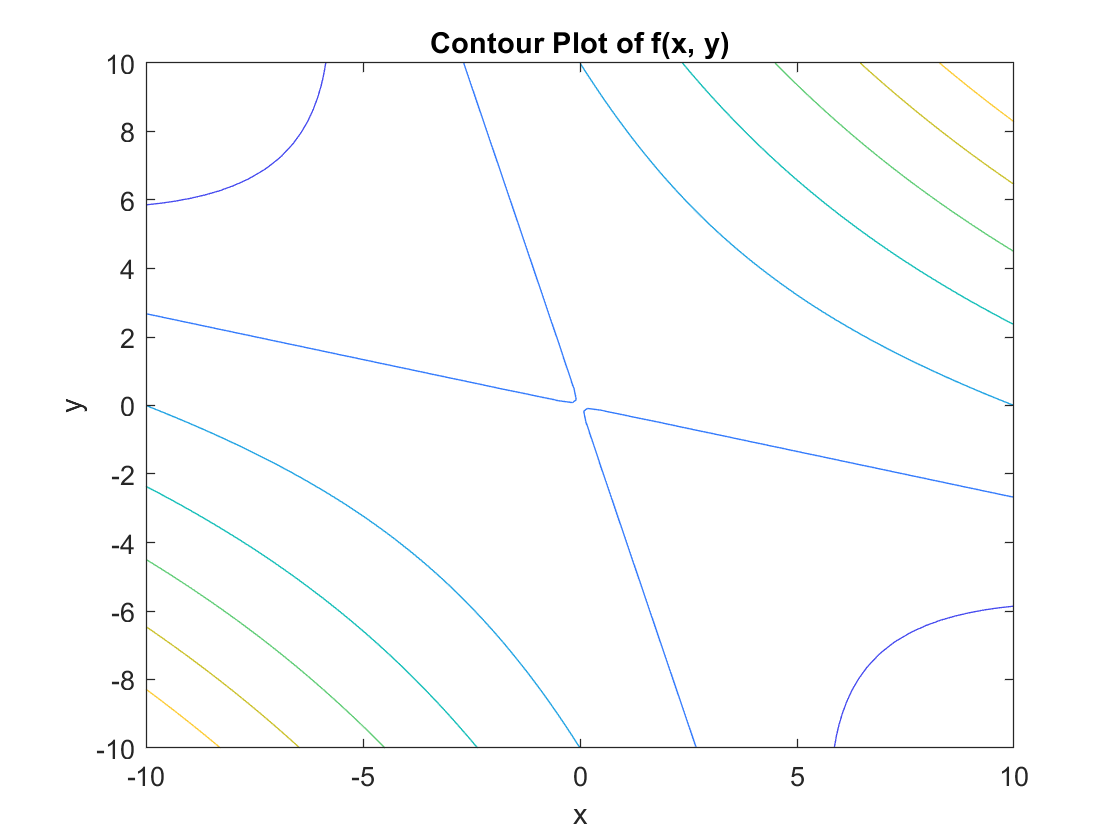
\includegraphics[width=0.5\textwidth]{Problem1_Contour.png} \end{center}
\noindent \\The generic quadratic function form is: ${F(x) = c + d^Tx + \frac{1}{2}x^TAx}$ \\ \\We can write our function in this form: \\ \\
  $f(x,y) =
  \frac{1}{2}
  \begin{bmatrix}
    x & y
  \end{bmatrix}
  \begin{bmatrix}
    2 & 4 \\
    4 & 2
  \end{bmatrix}
  \begin{bmatrix}
    x \\
    y
  \end{bmatrix}
  $,
  where $ x = 
  \begin{bmatrix}
    x \\
    y
  \end{bmatrix}$
  and A is the symetric matrix $A =   
  \begin{bmatrix}
    2 & 4 \\
    4 & 2
  \end{bmatrix}$. \\ 

  \noindent \\ The gradient is $\nabla f=
  \begin{bmatrix}
    \frac{\partial f}{\partial x} \\
    \frac{\partial f}{\partial y}
  \end{bmatrix} =
  \begin{bmatrix}
    2x+4y \\
    4x+2y
  \end{bmatrix}
  $. \\\\ \\In order to find the local minima/maxima we set the gradient equal to zero: \\ \\$\nabla F=0 \Rightarrow 
  \begin{bmatrix}
    2x+4y \\
    4x+2y
  \end{bmatrix} =
  \begin{bmatrix}
    0 \\ 0
  \end{bmatrix} \Rightarrow x=0$ and $y=0
  $\\ \\ \\
  So f(0,0) is a critical point. In order to determine if it is a local minimum or a maximum we need to calculate the eigenvalues of A:\\ \\
  ${det(A - \lambda*I)} = \det \left ( \begin{bmatrix}
    2 & 4 \\
    4 & 2
  \end{bmatrix} 
  -\begin{bmatrix}
    \lambda & 0 \\
    0 & \lambda
  \end{bmatrix} \right )  = 
  \det \left (\begin{bmatrix}
    2-\lambda & 4 \\
    4 & 2-\lambda
\end{bmatrix} \right ) = (2-\lambda)(2-\lambda)-16=\\ \\4-4\lambda+\lambda^2-16=\lambda^2-4\lambda-12$ 
So $\lambda = -2 $ or $\lambda = 6$. \\ \\
The eigenvalues have opposite signs, so the critical point f(0,0) is a Saddle point and the function has no minimum or maximum.






%Problem 2
\newpage
\noindent \textbf{Problem 2}

\noindent Execute two iterations of the Gradient Descent to the function: $f(x_1,x_2) = (x_1+2x_2-7)^2 + (2x_1+ \\ x_2-5)^2$ with initial point: $x_0 = (-9.5,9.5)$. Show your analytic calculations
 using the optimal $b_0$ in \\ each iteration\\ \\ \\
\underline{\textbf{\textit{Solution:}}}

\noindent\\$\frac{\partial f(x_1,x_2)}{\partial x_1} = 2(x_1+2x_2-7) + 4(2x_1+x_2-5)$, \hspace{1cm}  $\left. \frac{df}{dx_1} \right|_{x=x_0}= 5 - 58 = -53$
\\ \\ \\$\frac{\partial f(x_1,x_2)}{\partial x_2} = 4(x_1+2x_2-7) + 2(2x_1+x_2-5)$, \hspace{1cm}  $\left. \frac{df}{dx_2} \right|_{x=x_0}= 10 - 29 = -19$ \\ \\ \\ \\
\textbf{\textit{First iteration:}}
\\ The gradient at $x_0 = (-9.5,9.5)$ is: \, $\nabla f(x_0) = [-53, -19]$ \\ \\Thus, \, $\|\nabla f(x_0)\| = \sqrt{(-53)^2+(-19)^2} \approx 56.3$
\\ \\The direction of descending is: \, $s_0 = -\frac{\nabla f(x_0)}{\|\nabla f(x_0)\|} \approx [0.94, 0.34]$
\\ \\ \\ \\In order to find the optimal $b_0$ we'll take the derivative $\frac{\partial f(x_0')}{\partial b_0}$ and set it to 0. Knowing that $x_0' = x_0 + b_0s_0$ the value of 
$f(x_0')$ is: \\ \\ $f(x_0+b_0s_0) = f(-9.5+0.94b_0, 9.5+0.34b_0) = (-9.5+0.94b_0+19+0.68b_0-7)^2 + (-19+1.88b_0+9.5+0.34b_0-5)^2 = (2.5 + 1.62b_0)^2 + (-14.5+2.22b_0)^2$\\ \\ 
\\ So the optimal $b_0$ is: \\ \\$\frac{\partial f(x_0+b_0s_0)}{\partial b_0} = 0 \Rightarrow 2*1.62(2.5+1.62b_0) + 2*2.22(-14.5+2.22b_0) = 0 \Rightarrow \\ \\
\Rightarrow -56.28 +15.11b_0 = 0 \Rightarrow \bm{b_0 \approx 3.72}$ \, and \, $\bm{x_0' \approx [-6,10.76]}$\\ \\ \\



\noindent \textbf{\textit{Second iteration::}}
\\ \\ $\left. \frac{df}{dx_1} \right|_{x=x_0'}= 17.04 - 24.968 = -7.92$ \\ \\ \\$\left. \frac{df}{dx_2} \right|_{x=x_0'}= 34.08 - 12.48 = 21.6$
\\ \\ \\ \\The gradient at $x_0' = (-6,10.76)$ is: \, $\nabla f(x_0') = [-7.92, 21.6]$ \\ \\Thus, \, $\|\nabla f(x_0)\| = \sqrt{(-7.92)^2+(21.6)^2} \approx 23$
\\ \\The direction of descending is: \, $s_0' = -\frac{\nabla f(x_0')}{\|\nabla f(x_0')\|} \approx [0.34, -0.94]$
\\ \\ \\ \\In order to find the optimal $b_0'$ we'll take the derivative $\frac{\partial f(x_0'')}{\partial b_0}$ and set it to 0. Knowing that $x_0'' = x_0' + b_0's_0'$ the value of 
$f(x_0'')$ is: \\ \\ $f(x_0'+b_0's_0') = f(-6+0.34b_0', 10.76-0.94b_0') = (-6+0.34b_0'+21.52-1.88b_0'-7)^2 + (-12+0.68b_0'+10.76-0.94b_0'-5)^2 = (8.52-1.54b_0')^2 + (-6.24-0.26b_0')^2$\\ \\ 
\\ So the optimal $b_0'$ is: \\ \\$\frac{\partial f(x_0'+b_0's_0')}{\partial b_0'} = 0 \Rightarrow 2(-1.54)(8.52-1.54b_0') + 2(-0.26)(-6.24-0.26b_0') = 0 \Rightarrow \\ \\
\Rightarrow -22.99 +4.88b_0' = 0 \Rightarrow \bm{b_0' \approx 4.71}$ \, and \, $\bm{x_0'' \approx [-4.4,15.19]}$\\

%Problem 3
\newpage
\noindent \textbf{Problem 3}
\\ \\
Consider the dynamical system called Henon map defined by the following recursive equation:
\begin{center}
  ${x_k+1 = f(x_k) = 1-ax_k^2+bx_{k-1}}$.
\end{center}
Many dynamical systems transition into chaos as we increase a control or gain parameter
such as ${x_0}$. Select (a,b)=(0.3, 0.4) and use the two choices of initial conditions, $x_0$=0 and
$x_0$=0.00001, to generate $x_1$,…. Plot the two trajectories. Are they aperiodic (chaotic) or
periodic? For the series of the following questions, we need to plot the sequence of
generated values and also record your observations.
\begin{enumerate} [label=\Alph*]
  \item $[x_0=0]$ Test the generated sequence of $x_i$ with b=0, and various values for a. 
              What doyou observe? chaos or some fixed-point(s)?
  \item Test for various values of $x_0$ and b, but a being between 0 and 0.32
  \item $[x_0=0]$ Test the case of values (a,b)=(0.3675, 0.3). What do you observe?
  \item $[x_0=0]$  Test the case of values (a,b)=(0.2, 0.4), (a,b)=(0.5, 0.4) and (a,b)=(0.9, 0.4). What do you observe?
\end{enumerate}
\noindent \\ \\ 
\underline{\textbf{\textit{Solution:}}}
\begin{enumerate} [label=\Alph*]
  \item Testing the generated sequence of $x_i$ with b = 0, and various values for a, we observed some fixed points following a repeating pattern. Here are some examples: 
    \\ \\

    \begin{figure}[h]
      \centering
      \begin{minipage}[t]{0.5\textwidth}
        \centering
        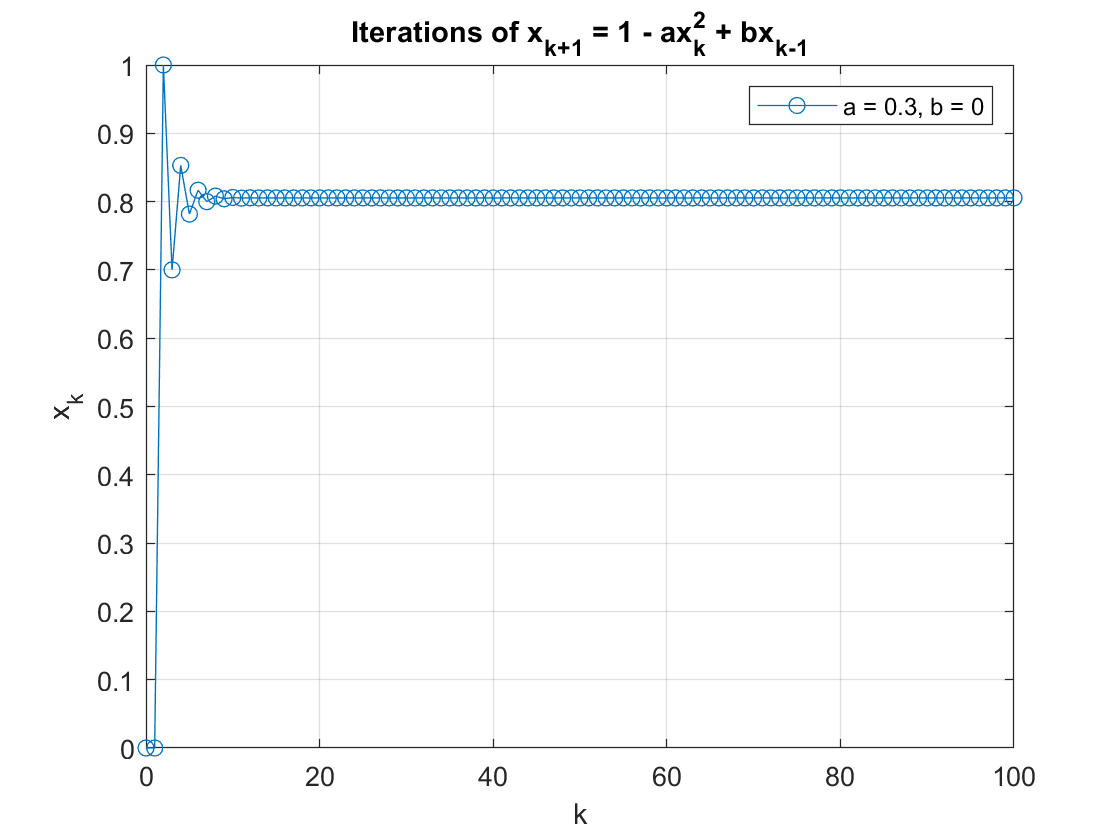
\includegraphics[width=0.8\linewidth]{Problem3_a0.3.png}
        \caption{a=0.3}
        \label{fig:img1}
      \end{minipage}%
      \begin{minipage}[t]{0.5\textwidth}
        \centering
        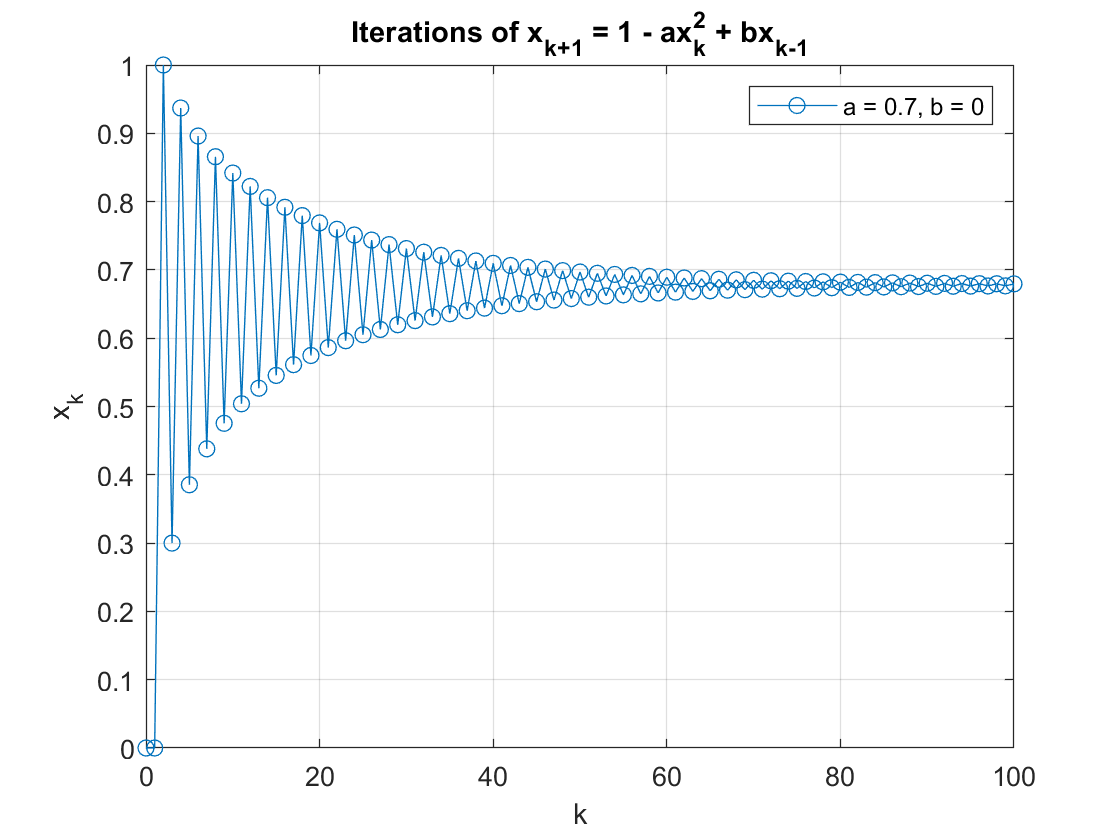
\includegraphics[width=0.8\linewidth]{Problem3_a0.7.png}
        \caption{a=0.7}
        \label{fig:img2}
      \end{minipage}
    \end{figure}

    \begin{figure}[h]
      \centering
      \begin{minipage}[t]{0.5\textwidth}
        \centering
        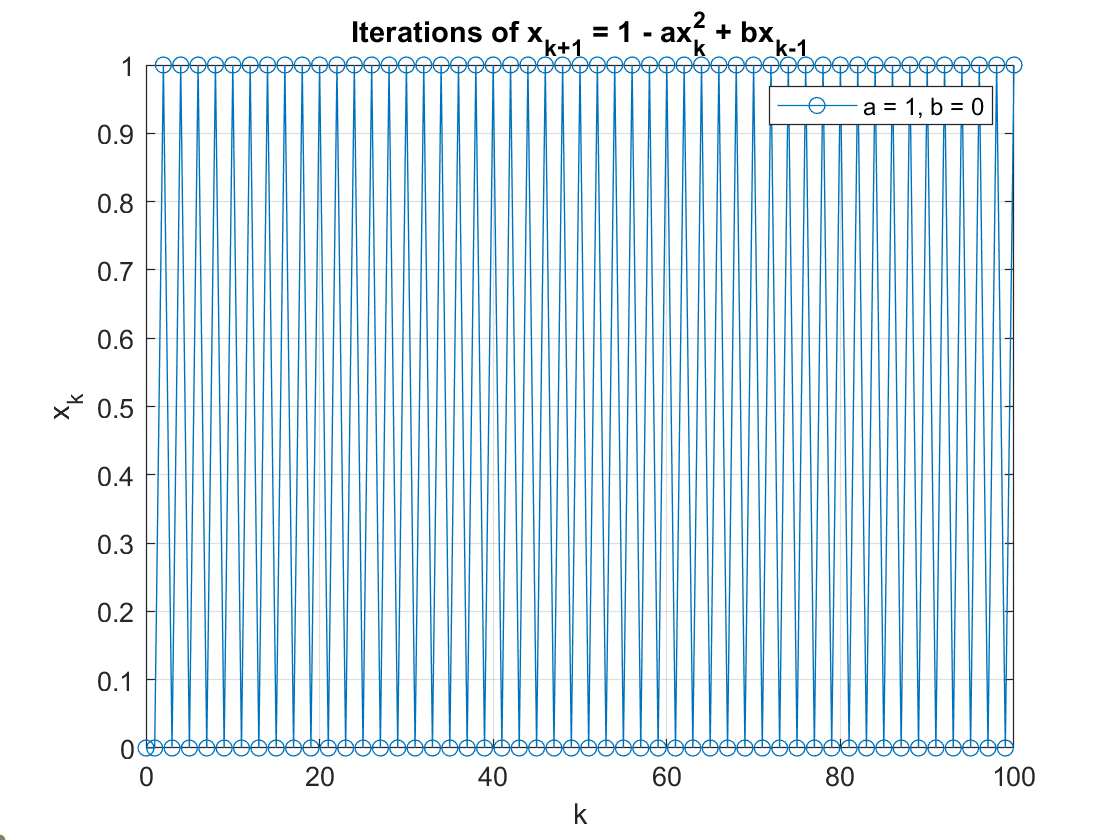
\includegraphics[width=0.8\linewidth]{Problem3_a1.png}
        \caption{a=1}
        \label{fig:img1}
      \end{minipage}%
      \begin{minipage}[t]{0.5\textwidth}
        \centering
        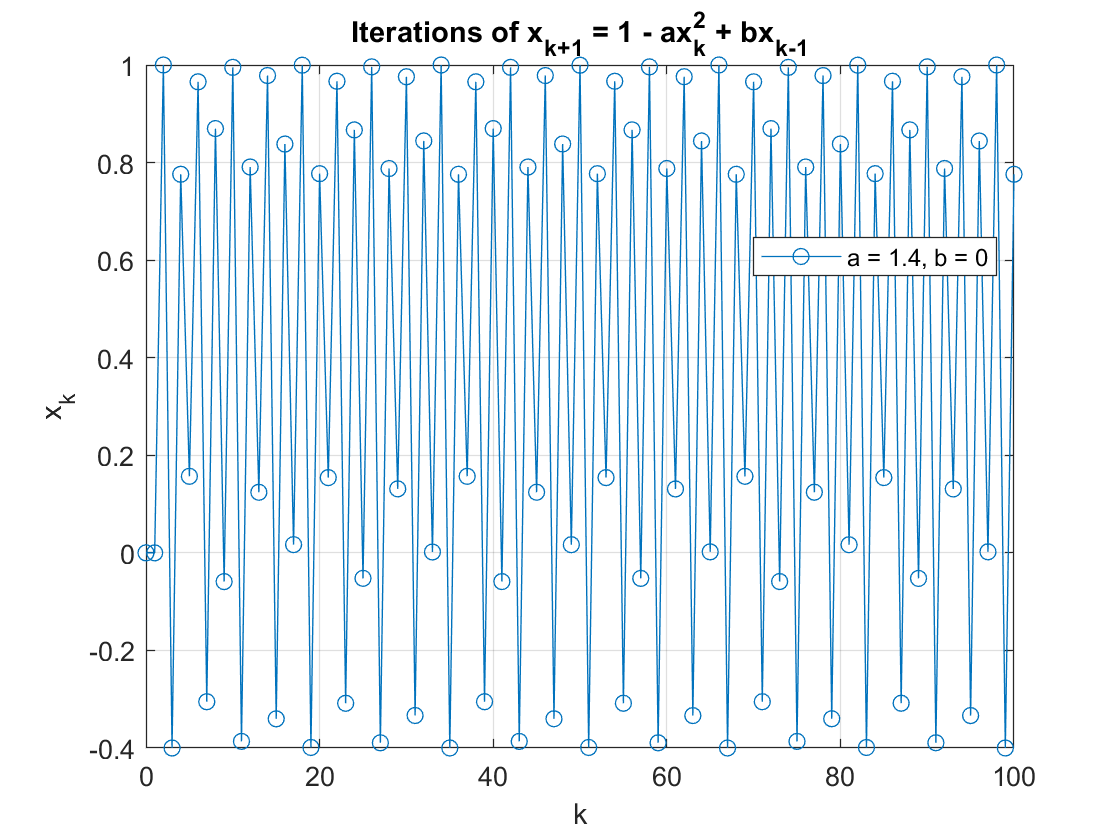
\includegraphics[width=0.8\linewidth]{Problem3_a1.4.png}
        \caption{a=1.4}
        \label{fig:img2}
      \end{minipage}
    \end{figure} 
    
    \begin{figure}[h]
      \centering
      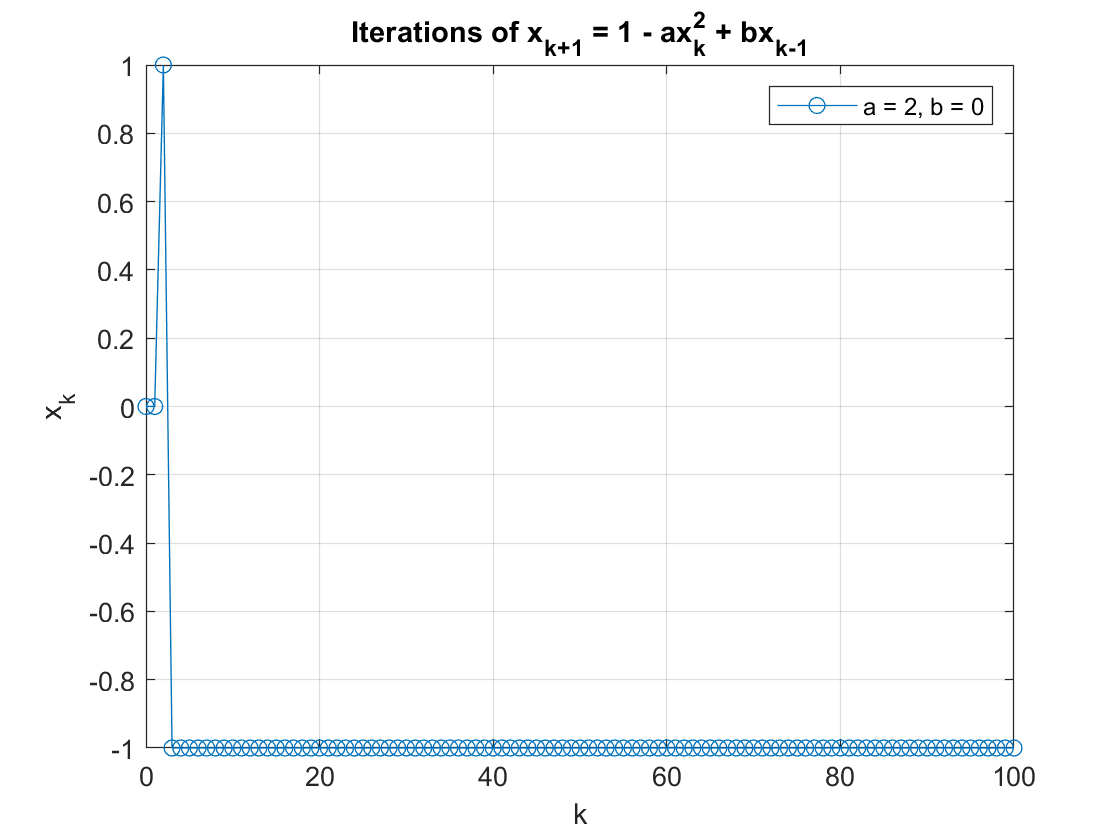
\includegraphics[width=0.45\textwidth]{Problem3_a2.png}
      \caption{a = 2}
      \label{fig:a2}
    \end{figure}

  \newpage
  \item Testing for various values of $x_0$ and b with a being between 0 and 0.32:
  \begin{figure}[h]
    \centering
    \begin{minipage}[t]{0.5\textwidth}
      \centering
      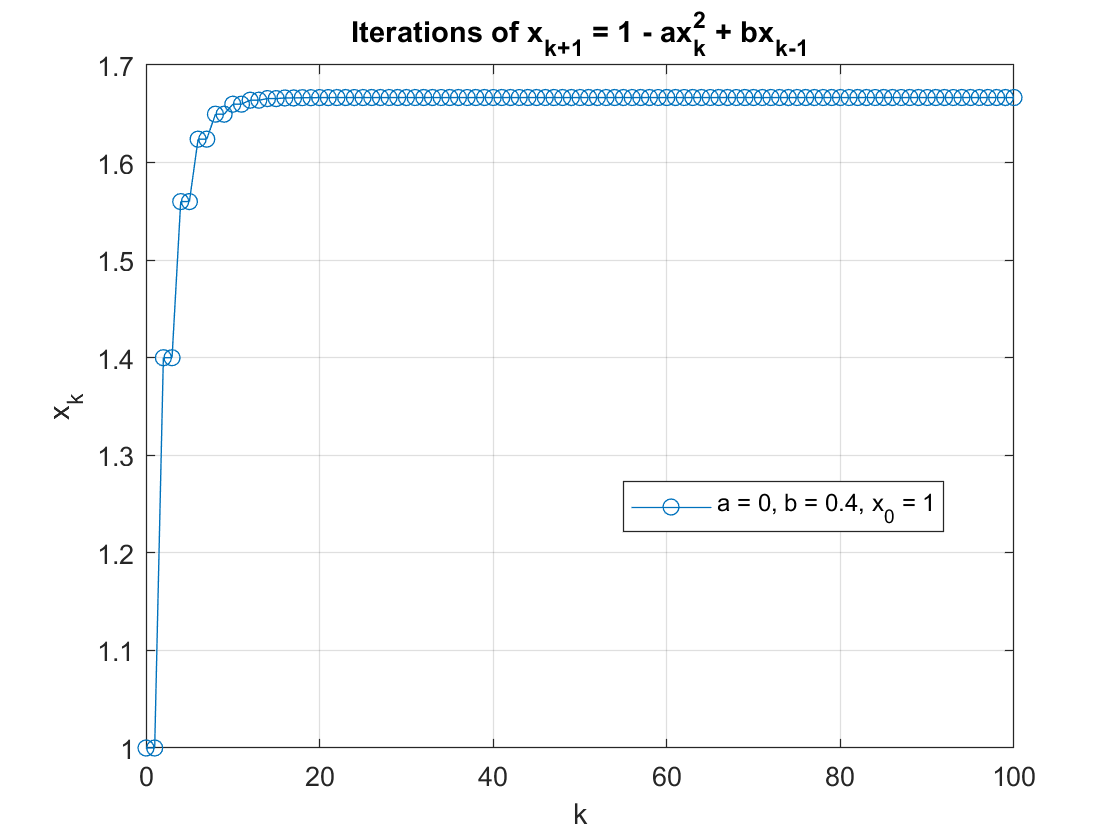
\includegraphics[width=0.8\linewidth]{Problem3_B_1.png}
      \caption{a=0, b=0, $x_0$=1} 
      \label{fig:img1}
    \end{minipage}%
    \begin{minipage}[t]{0.5\textwidth}
      \centering
      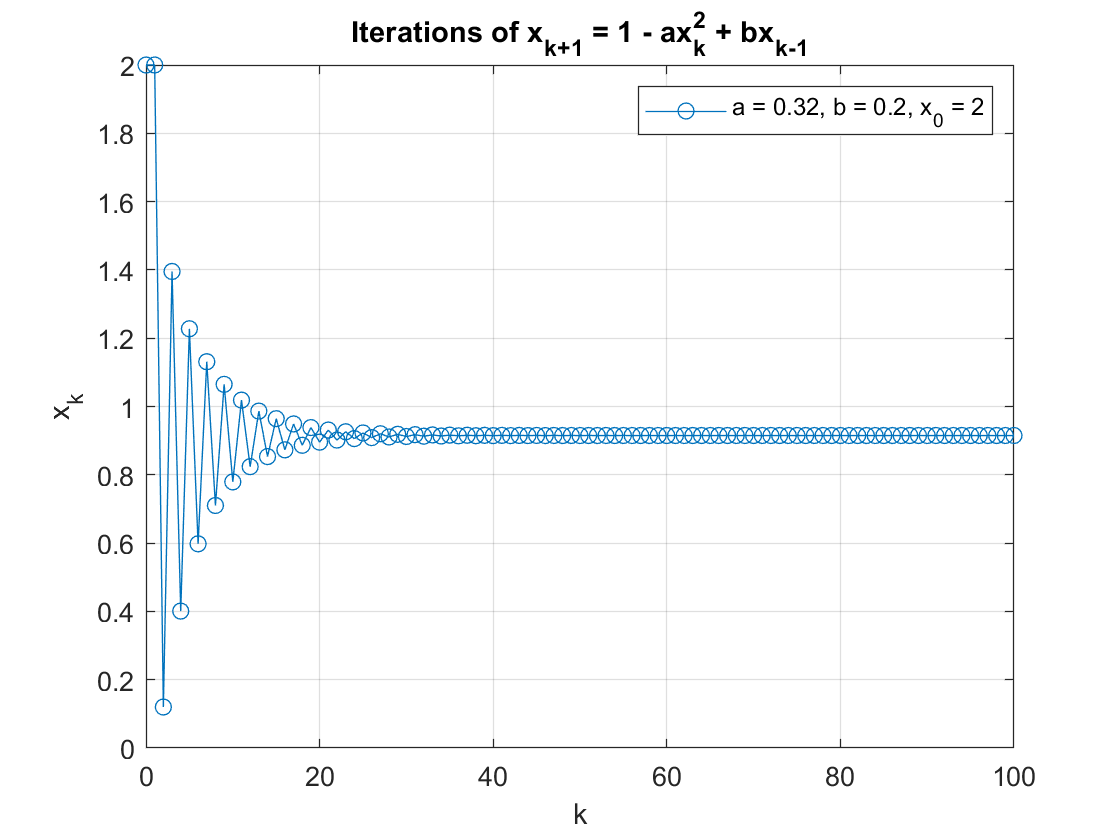
\includegraphics[width=0.8\linewidth]{Problem3_B_2.png}
      \caption{a=0.32, b=0.2, $x_0$=2}
      \label{fig:img2}
    \end{minipage}
  \end{figure}
  \begin{figure}[H]
    \centering
    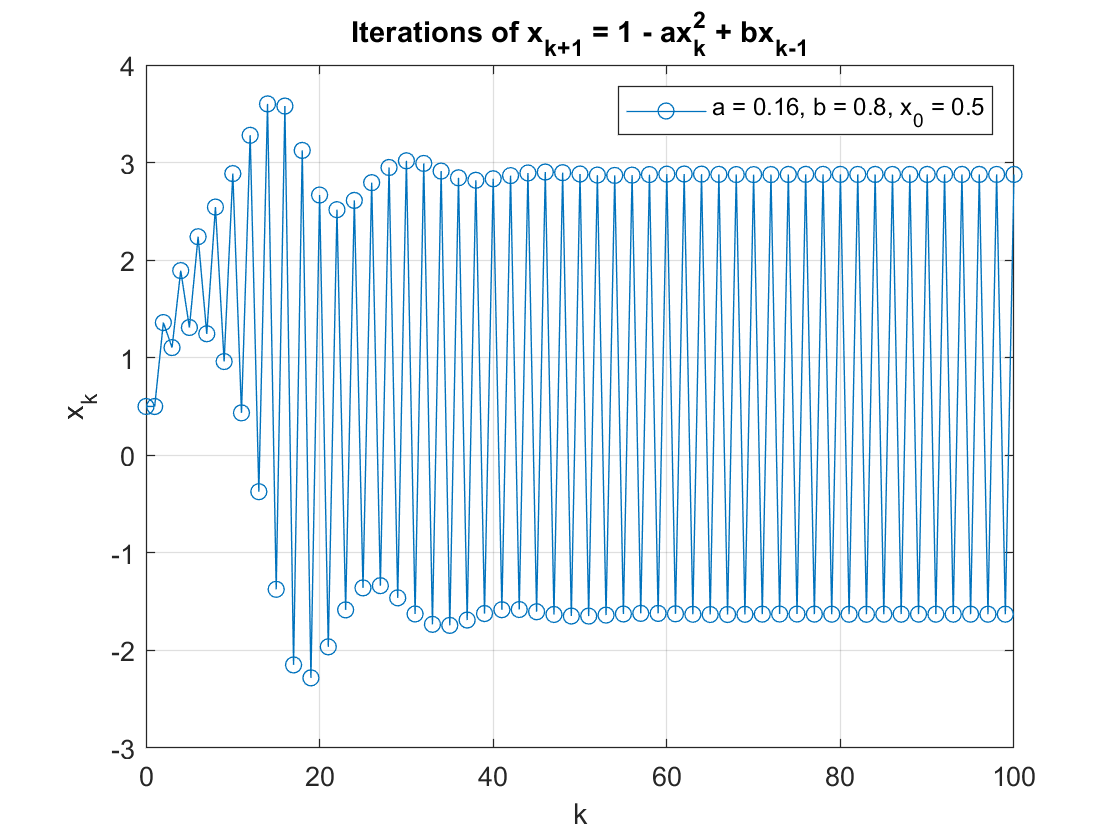
\includegraphics[width=0.45\textwidth]{Problem3_B_3.png}
    \caption{a=0.16, b=0.8, $x_0$=0.5}
    \label{fig:a2}
  \end{figure}

  \clearpage 
  \item We observe that the points reapeat at a smaller width with each repetition:
  \begin{figure}[H]
    \centering
    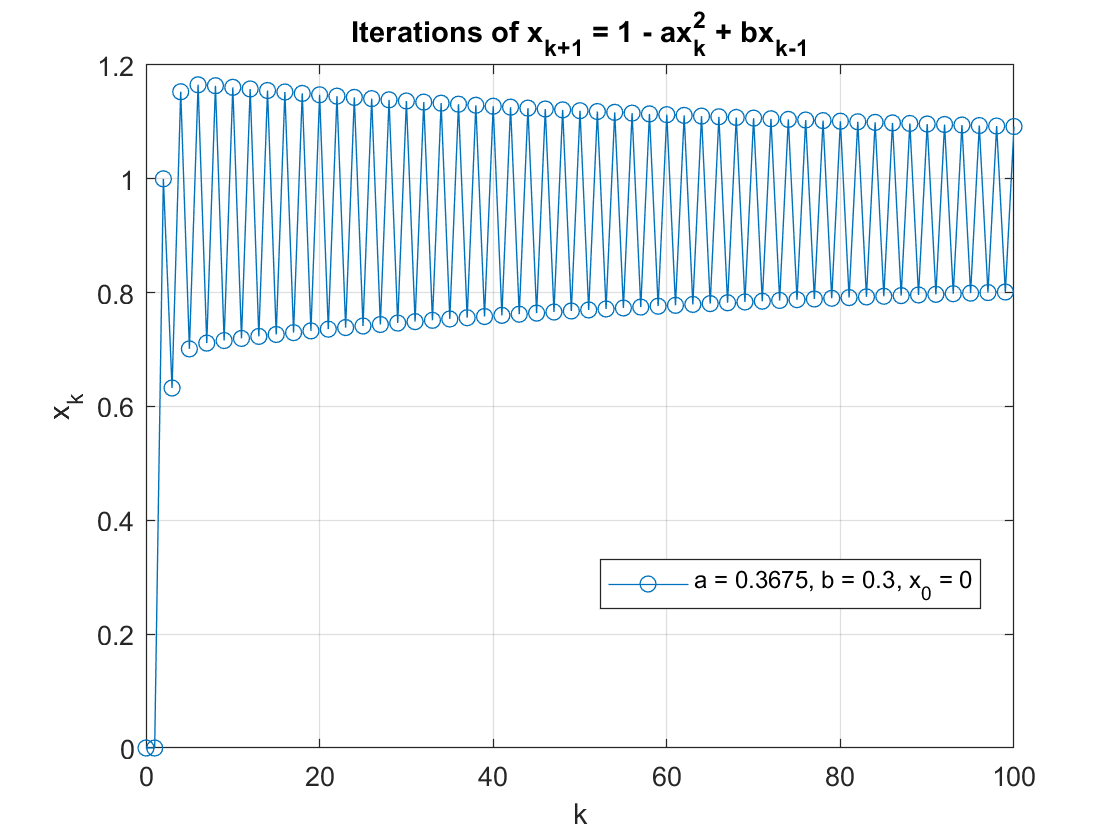
\includegraphics[width=0.45\textwidth]{Problem3_C.png}
    \caption{a=0.3675, b=0.3, $x_0$=0}
    \label{fig:a2}
  \end{figure}

  
  \item We observe that the for each of the value pairs the points start at a different width that slowly decreases:
  
  \begin{figure}[h]
    \centering
    \begin{minipage}[t]{0.5\textwidth}
      \centering
      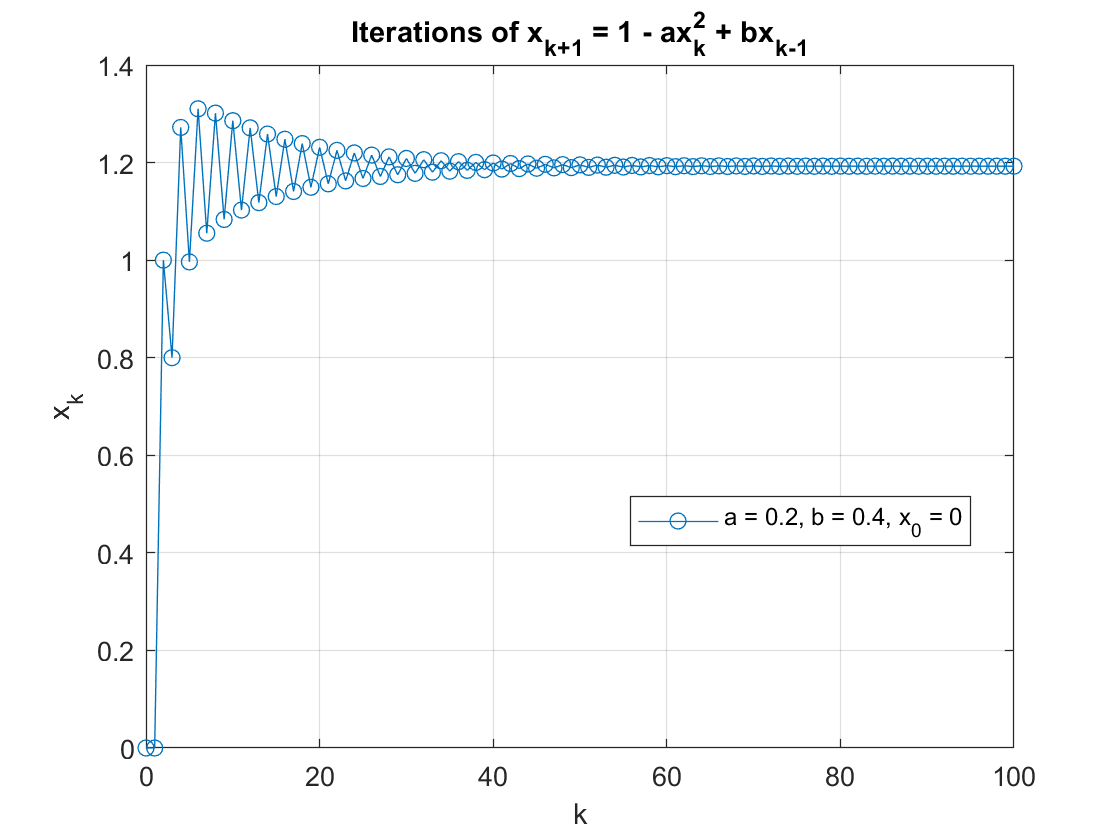
\includegraphics[width=0.8\linewidth]{Problem3_D_1.png}
      \caption{a=0.2, b=0.4, $x_0$=0} 
      \label{fig:img1}
    \end{minipage}%
    \begin{minipage}[t]{0.5\textwidth}
      \centering
      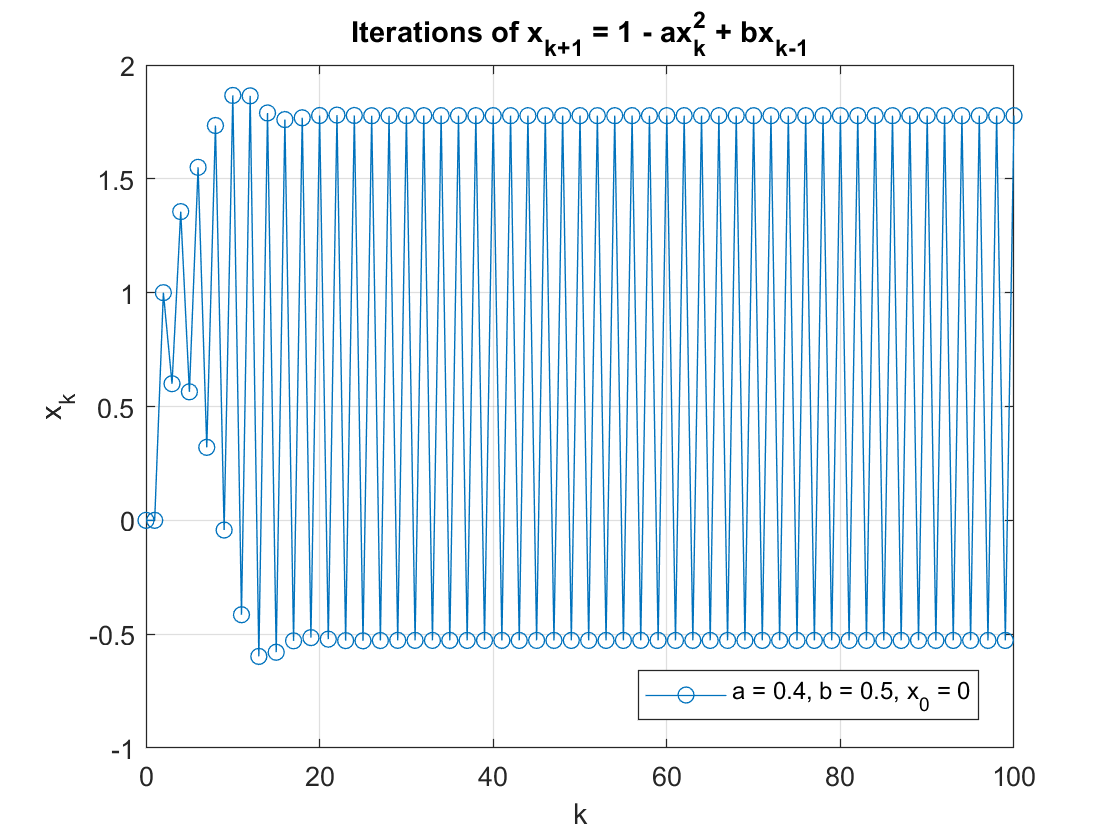
\includegraphics[width=0.8\linewidth]{Problem3_D_2.png}
      \caption{a=0.4, b=0.5, $x_0$=0}
      \label{fig:img2}
    \end{minipage}
  \end{figure}
  \begin{figure}[H]
    \centering
    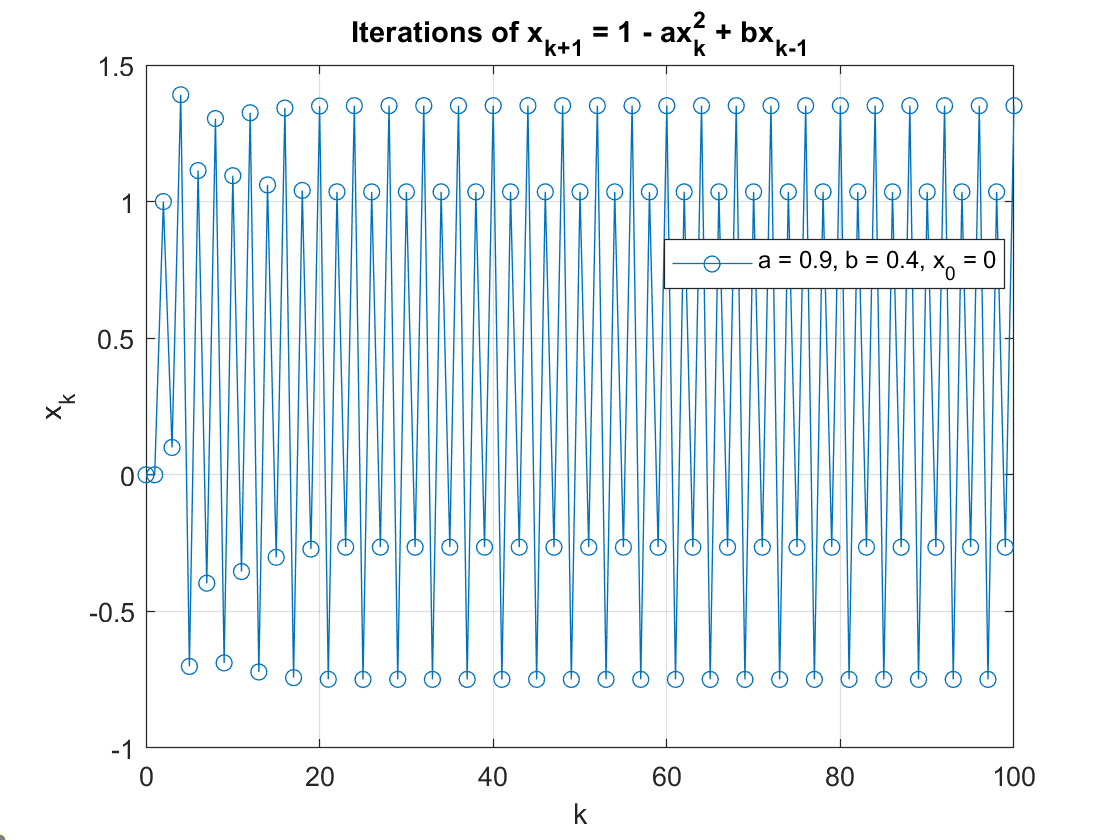
\includegraphics[width=0.45\textwidth]{Problem3_D_3.png}
    \caption{a=0.9, b=0.4, $x_0$=0}
    \label{fig:a2}
  \end{figure}
\end{enumerate}


%Problem 4
\newpage
\noindent \textbf{Problem 4}

\noindent Express the derivative dS/dx, denoted as S', of the following activation functions S in terms of the \\ original function S, i.e., determine ${\phi}$ such that S' = ${\phi}$(S,x). 
[The first three functions comprise well-\\established activation functions, known as logsig, tansig, and Google's Swish, respectively]. In particular, for the fourth activation
function, recognize the relation of its derivative to the Swish activation function.\\
\begin{enumerate}
  \item $S = \frac{1}{1+e^{-x}}$ \\
  \item $S = \frac{e^{x}-e^{-x}}{e^{x}+e^{-x}}$ \\
  \item $S = \frac{x}{1+e^{-x}}$ \\
  \item $S = x*(tanh(ln(1+e^{x})))$ \\
\end{enumerate}
\noindent \\ \\ 
\underline{\textbf{\textit{Solution:}}}

\begin{enumerate}
  \item $S' = (\frac{1}{1+e^{-x}})' = -\frac{1}{(1+e^{-x})^2}(-e^{-x}) = \frac{e^{-x}}{(1+e^{-x})^2} \Rightarrow S' = \frac{1}{1+e^{-x}} * \frac{1}{1+e^{-x}} * e^{-x}$ \hspace{0.5cm} [a] \\ \\
    We know that $S = \frac{1}{1+e^{-x}} \Rightarrow 1+e^{-x} = \frac{1}{S}  \Rightarrow e^{-x} = \frac{1-S}{S}$ \hspace{3.2cm} [b]\\ \\ Using [b] on [a] we get: \\ \\
    $S' = f(S,x) = S * S * \frac{1-S}{S} \Rightarrow \bm{S' = S(1-S)}$ \\ \\
  \item $S' = (\frac{e^{x}-e^{-x}}{e^{x}+e^{-x}})' = \frac{(e^{x}+e^{-x})(e^{x}+e^{-x}) - (e^{x}-e^{-x})(e^{x}-e^{-x})}{(e^{x}+e^{-x})^2} = \frac{(e^{x}+e^{-x})^2 - (e^{x}+e^{-x})^2}{(e^{x}+e^{-x})^2}
    = 1 - \frac{(e^{x}-e^{-x})^2}{(e^{x}+e^{-x})^2}$ \\ \\ So, $S' = f(S,x) \Rightarrow \bm{S' = 1 - S^2}$ \\ \\
  \item Knowing that $s(x) = \frac{1}{1+e^{-x}}$ is the sigmoid function, we can write S as: \\ \\ $S = xs(x)$ \hspace{0.3cm} [c], \hspace{0.3cm} and S' as: $S' = (\frac{x}{1+e^{-x}})' = (xs(x))' = s(x) + xs'(x)$ 
  \hspace{1cm} [d] \\ \\In (1) we prooved that s'(x) = s(x)(1-s(x)). By using that on [d] we get: \\ \\ $S' = s(x) + x(s(x)(1-s(x))) = xs(x) + s(x) -xs^2(x) = xs(x) + s(x)(1-xs(x))$ \\ \\ From [c] we know that 
  $S = xs(x) \Rightarrow s(x) = \frac{S}{x}$. \\ \\ So, $S' = f(S,x) \Rightarrow \bm{S' = S + \frac{S}{x}(1-S)}$\\ \\
  \item $S' = (x*(tanh(ln(1+e^{x}))))' = tanh(ln(1+e^{x})) + x(tanh(ln(1+e^{x})))'$ \\ \\ Knowing that $tanh(u) = \frac{e^{u}-e^{-u}}{e^{u}+e^{-u}}$ is the tansig function and having calculated it's derivative \\ 
  in (2), we know that $(tanh(u))' = 1 - tanh^2(u)$. By using this information together with the chain rule we get: \\ \\ $S' = tanh(ln(1+e^{x})) + x(1 - tanh^2(ln(1+e^{x}))(ln(1+e^{x}))')$ \hspace{0.5cm} [e] \\ \\ \\
  Let's calculate the derivative of $ln(1+e^{x})$: \\ \\$(ln(1+e^{x}))' = \frac{1}{1+e^{x}}e^x = \frac{1}{1+\frac{1}{e^x}} = \frac{1}{1+e^-x} = s(x)$ (sigmoid function)\hspace{0.3cm} [f]\\ \\ \\We also know that
  $tanh(u) = 2s(2u)-1$ \hspace{0.3cm} [g]. \\ \\ Knowing that Swish = xs(x) and using [f] and [g] on [e] we get: \\ \\ \\$S' = (Swish,x) = tanh(ln(1+e^{x})) + x(1 - tanh^2(ln(1+e^{x}))s(x)) =\\ \\ tanh(ln(1+e^{x})) + xs(x) - xs(x)tanh^2(ln(1+e^{x}))
  \Rightarrow \\ \\{S' = Swish*(1 - tanh^2(ln(1+e^{x}))) +tanh(ln(1+e^{x})) \Rightarrow}$ \\ \\$\bm{S' = Swish*(1-\frac{S^2}{x^2}) + \frac{S}{x}}$
\end{enumerate}

%Problem 5
\newpage
\noindent \textbf{Problem 5}

\noindent Consider the following neural network \\ \\
\begin{figure}[h]
  \centering
  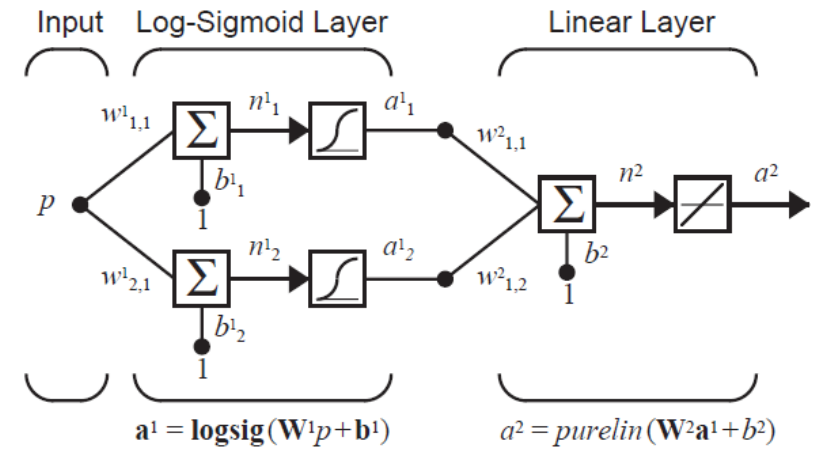
\includegraphics[width=0.4\textwidth]{pr5_a.png}
  
\end{figure}

\noindent with $w^1_{1,1} = -2, w^1_{2,1} = -1, b^1_1 = -0.5, b^1_2 = -0.75, w^2_{1,1} = 2, w^2_{1,2} = 1, b^2 = 0.5$. 
Sketch the following responses (plot the indicated variable versus p for $-2 < p < 2$).
\begin{enumerate}[label=\Alph*]
  \item $a^1_1$
  \item $a^1_2$
  \item $a^2$
\end{enumerate}

\noindent \\Then, change the logsig activation function with the Swish activation function and sketch 
again the aforementioned responses. \\ \\

\noindent \underline{\textbf{\textit{Solution:}}}
\begin{figure}[h]
  \centering
  \begin{minipage}[t]{0.5\textwidth}
    \centering
    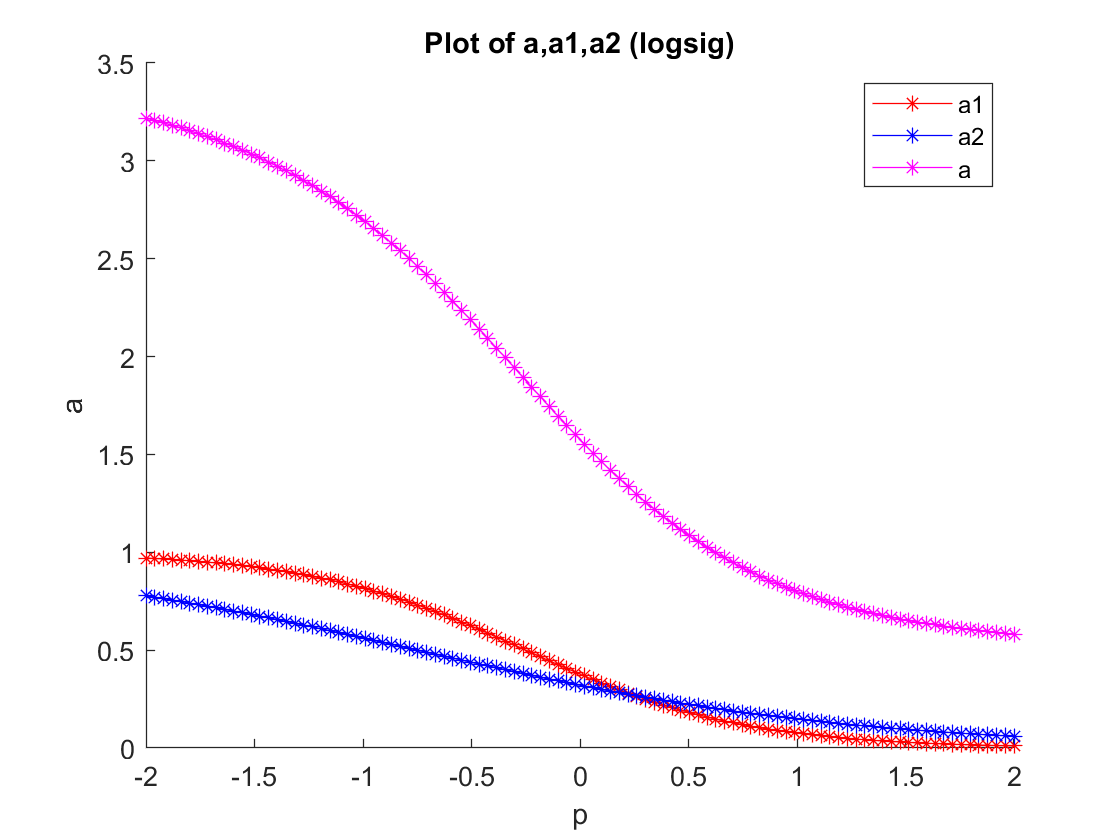
\includegraphics[width=0.8\linewidth]{Problem5_logsig_all.png}
    \caption{logsig activation function} 
    \label{fig:img1}
  \end{minipage}%
  \begin{minipage}[t]{0.5\textwidth}
    \centering
    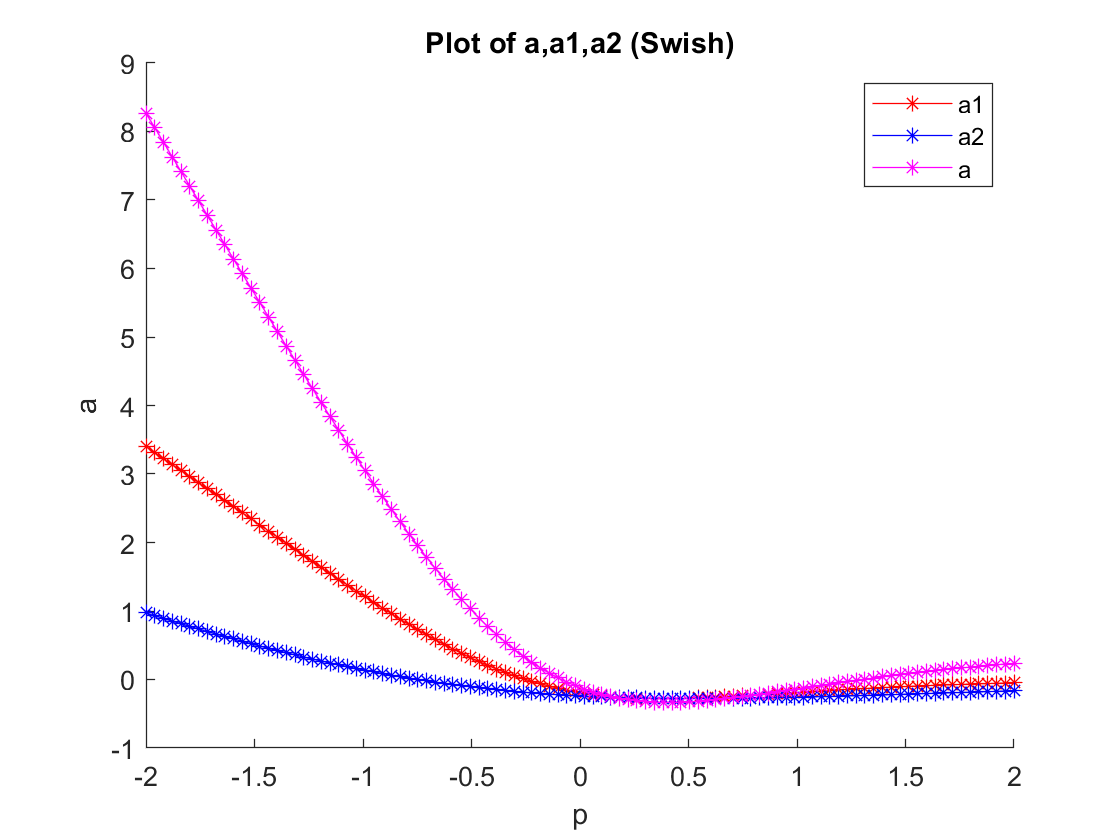
\includegraphics[width=0.8\linewidth]{Problem5_Swish_all.png}
    \caption{Swish activation function}
    \label{fig:img2}
  \end{minipage}
\end{figure}

%Problem 6
\newpage
\noindent \textbf{Problem 6}

\noindent We are interested in comparing the gradient descent optimizer for several values of the
batch size, i.e., $n_b=1\rightarrow$SGD, $n_b=n\rightarrow$GD, $n_b=\phi(n)<<n\rightarrow$BGD. While applying these
variants on a given problem with an objective function F, we observed that when $n_b=1$,
we get better convergence than $n_b=n$, while increasing the batch size from $n_b=1$ to
$n_b=n/10$ consistently improves the results, in that the method converges faster and to a
smaller value of the objective function F. We then observe that the convergence slows
down as we increase the batch size from n/10 to n.
Explain these observations. \\ \\

\noindent \underline{\textbf{\textit{Solution:}}}

\noindent \\Using SGD we get a better convergence than using GD because the smaller batch size means updating the model for each datapoint. 
This introduces randomness that can help escape from local minima thus getting a better convergence. 
GD uses the whole dataset and may get stuck at a local minima thus giving a worse convergence. 
Using 1/10 as the batch size is a good middle ground between SGD and GD allowing the method to escape the local minima while also providing a quick convergence.
However increasing the batch size further slows down the convergence because we have more datapoints to analyse and that makes each update smaller thus taking more time to converge.

%Problem 7
\newpage
\noindent \textbf{Problem 7}

\noindent You are given the following activation function:
\newline

\[S(x) = \begin{cases}
  x^k & \text{for } x > L \\
  x^k * \frac{(L+x)^m}{(L+x)^m + (L-x)^m} & \text{for } |x| \leq L \\
  0 & \text{for } x < -L
\end{cases}\]

\noindent where, k, L and m are trainable parameters, i.e., hyperparameters.
\begin{enumerate}[label=\Alph*]
  \item Show (graphically and analytically) how this activation function can approximate,
   Swish, sigmoid, ReLU, and ELU, i.e., by proper selection of hyperparameter values.
  \item Calculate the derivatives of S with respect to x, k, L and m. \\ \\
\end{enumerate}

\noindent \underline{\textbf{\textit{Solution:}}}

\begin{enumerate}[label=\Alph*]
  \item 
  \begin{enumerate}
  \item Swish: L = 2.8, k = 1, m = 1.2
  \begin{center} 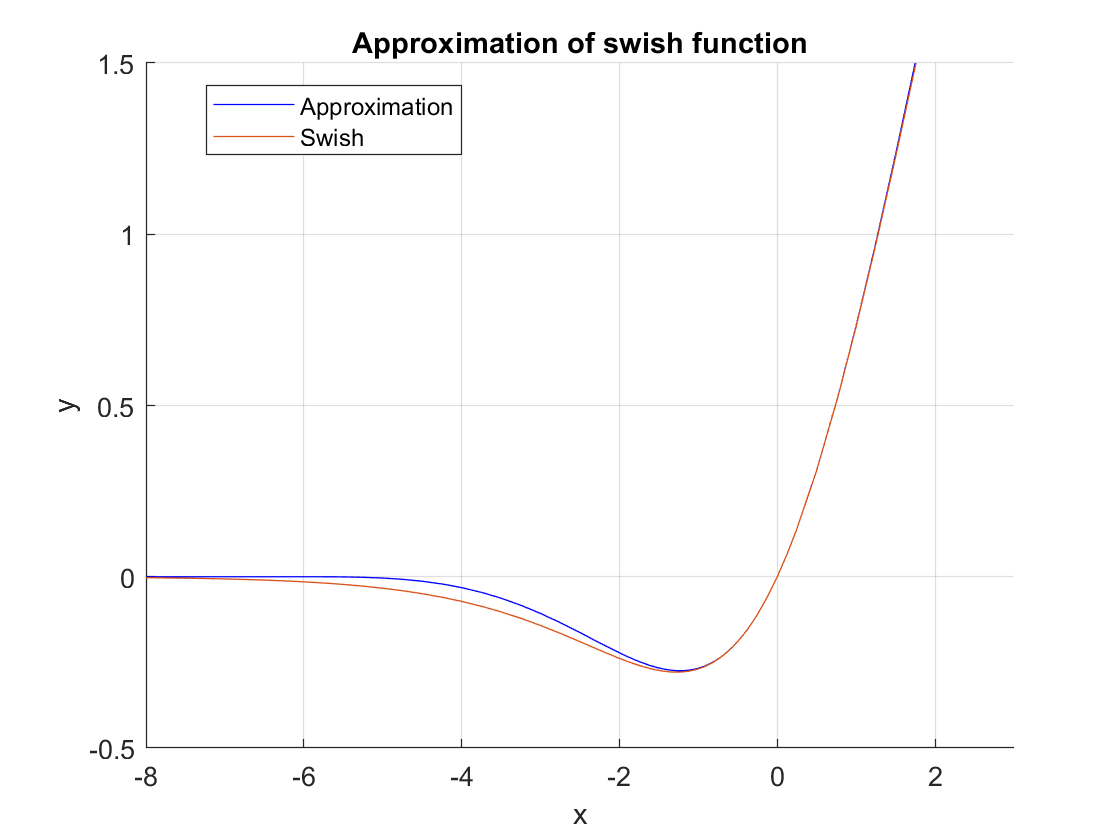
\includegraphics[width=0.8\textwidth]{Problem7_swish.png} \end{center} \newpage
  \item sigmoid: L = 5, k = 2.5, m = 0
  \begin{center} 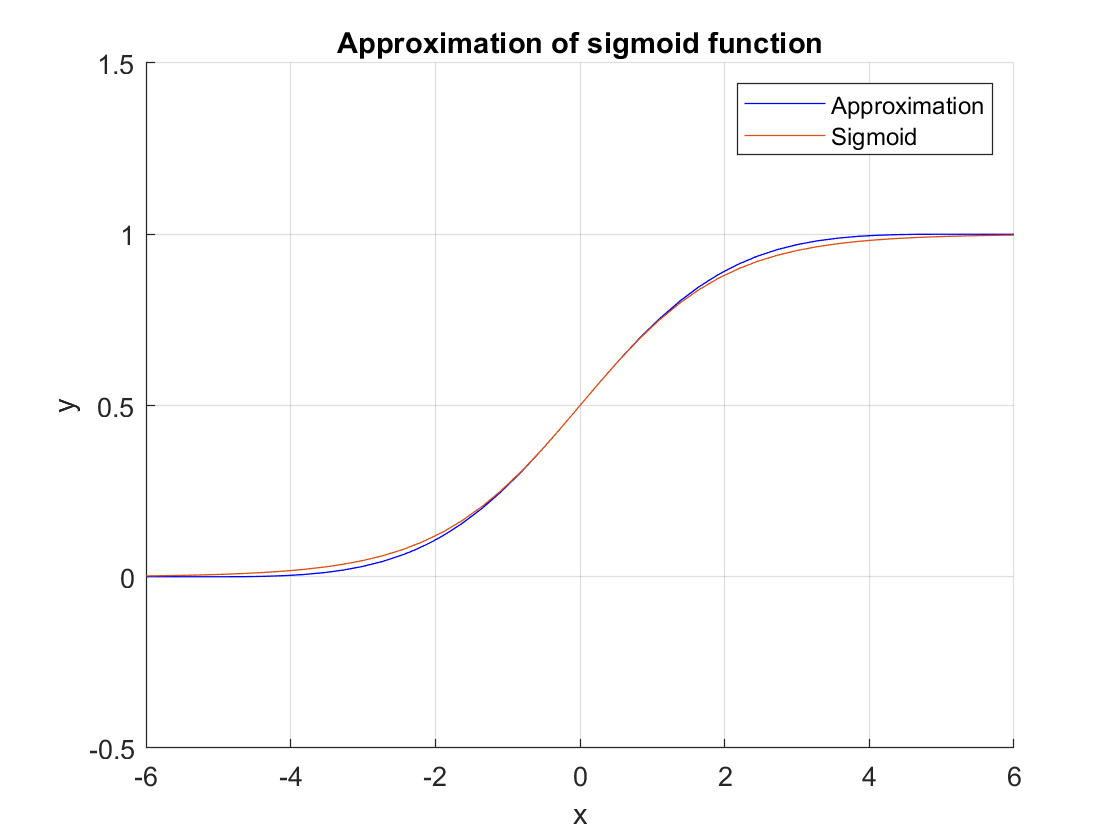
\includegraphics[width=0.8\textwidth]{Problem7_sigmoid.png} \end{center}
  \item ReLU: L = 0, k = 1, m is not relevant. \\ As we can see the apporoximation is so good the Relu function is not visible.
  \begin{center} 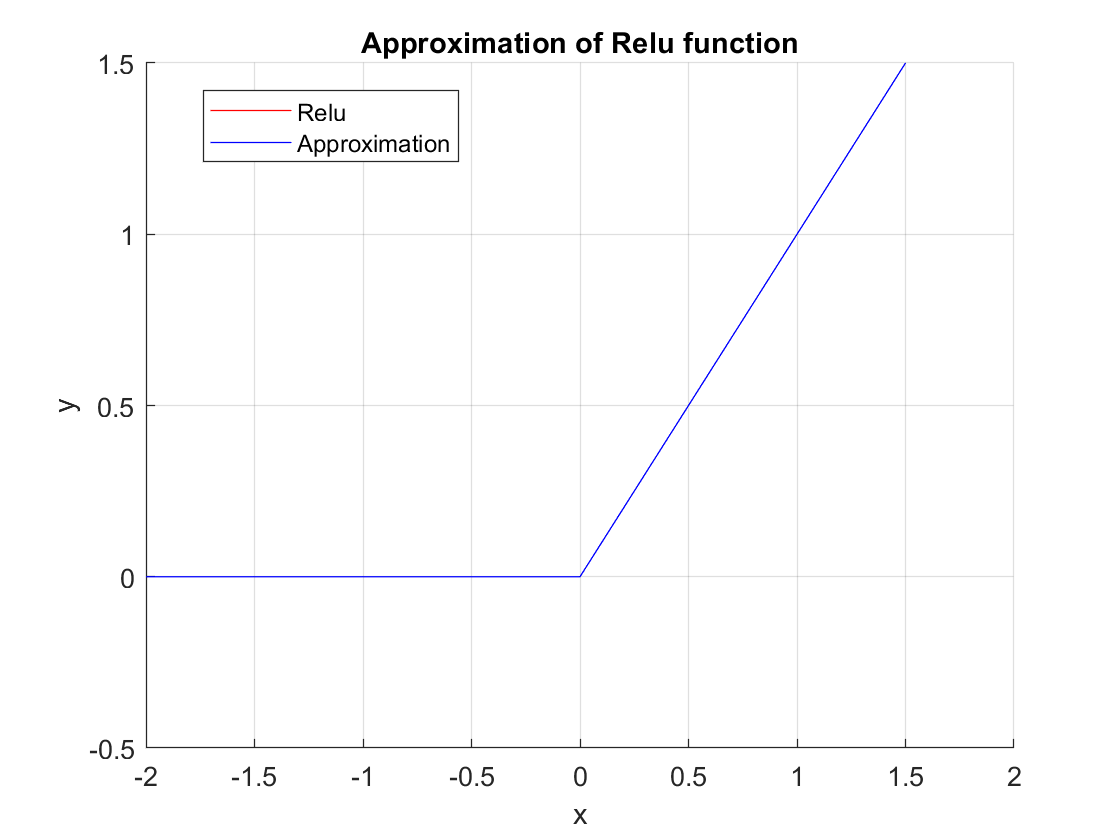
\includegraphics[width=0.8\textwidth]{Problem7_relu.png} \end{center}
  \newpage
  \item ELU: L = 50, k = 1, m = 6.5
  \begin{center} 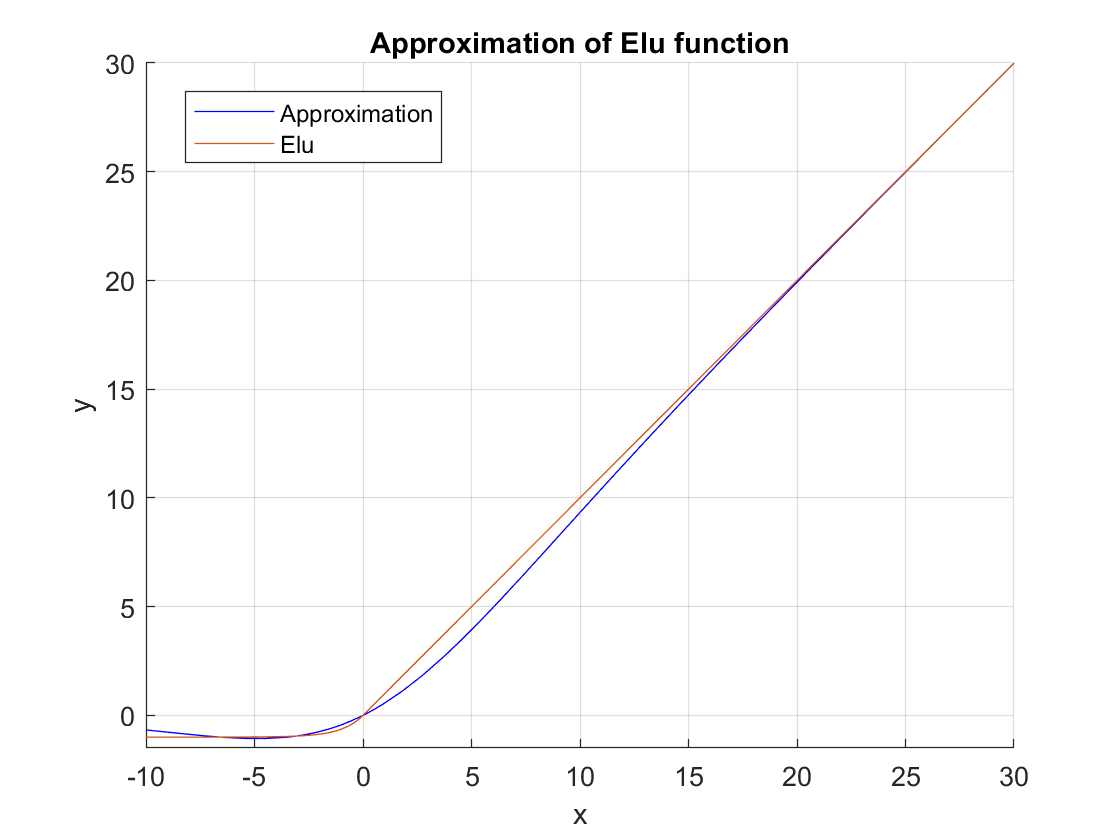
\includegraphics[width=0.8\textwidth]{Problem7_elu.png} \end{center}
  \end{enumerate}

  \item Derivative of S with respect to x: \\ \\
    \underline{For $x > L$:} \hspace{1.3cm} $S'(x) = kx^{(k-1)}$ \\ \\ \underline{For $x < -L$:} \hspace{1cm} $S'(x) = 0$ \\ \\ \underline{For $|x| \leq L$:} \\ \\ 
    $S'(x) = kx^{(k-1)} \frac{(L+x)^m}{(L+x)^m + (L-x)^m} + x^k * \frac{m(L+x)^{m-1}((L+x)^m + (L-x)^m) - (L+x)^m(m(L+x)^{m-1}-m(L-x)^{m-1})}{((L+x)^m + (L-x)^m)^2} \\ \\
    \\S'(x) = \frac{kx^{(k-1)}(L+x)^m((L+x)^m + (L-x)^m) + mx^k(L+x)^{m-1}((L+x)^m + (L-x)^m) - x^k(L+x)^m(m(L+x)^{m-1}-m(L-x)^{m-1})}{((L+x)^m + (L-x)^m)^2} \\ \\
    \\S'(x) = \frac{((L+x)^m + (L-x)^m)(kx^{(k-1)}(L+x)^m +mx^k(L+x)^{m-1}) - mx^k(L+x)^m((L+x)^{m-1} - (L-x)^{m-1})}{((L+x)^m + (L-x)^m)^2}$
    \\\\\\\\So, 
    \[\frac{\partial S(x)}{\partial x} = \begin{cases}
      kx^{(k-1)} & \text{for } x > L \\ \\
      \frac{((L+x)^m + (L-x)^m)(kx^{(k-1)}(L+x)^m +mx^k(L+x)^{m-1}) - mx^k(L+x)^m((L+x)^{m-1} - (L-x)^{m-1})}{((L+x)^m + (L-x)^m)^2} & \text{for } |x| \leq L \\ \\
      0 & \text{for } x < -L
    \end{cases}\]
    \newpage
    
    Derivative of S with respect to k: \\ \\ \underline{For $x > L$:} \hspace{1cm} $S'(x) = x^klnx$ \\ \\ \underline{For $x < L$:} \hspace{1cm} $S'(x) = 0$ \\ \\
    \underline{For $|x| \leq L$:} \hspace{0.8cm} $S'(x) = x^klnx* \frac{(L+x)^m}{(L+x)^m + (L-x)^m}$ \\ \\ \\ \\ So,
    \[\frac{\partial S(x)}{\partial k} = \begin{cases}
      x^klnx & \text{for } x > L \\ \\
      x^klnx* \frac{(L+x)^m}{(L+x)^m + (L-x)^m} & \text{for } |x| \leq L \\ \\
      0 & \text{for} x < -L
    \end{cases}\]\\ \\ \\ 
    \\ \\Derivative of S with respect to L: \\ \\ \underline{For $x > L$:} \hspace{1cm} $S'(x) = 0$\\\\ \underline{For $x < -L$:} \hspace{0.7cm}
    $S'(x) = 0$ \\ \\ \underline{For $|x| \leq L$:} \\ \\ $S'(x) = x^k * \frac{m(L+x)^{m-1}((L+x)^m + (L-x)^m) - (L+x)^m(m(L+x)^{m-1} + m(L-x)^{m-1})}{((L+x)^m + (L-x)^m)^2} \\ \\
    \\S'(x) = mx^k * \frac{(L+x)^{2m-1} + (L+x)^{m-1}(L-x)^m - (L+x)^{2m-1} - (L+x)^m(L-x)^{m-1}}{((L+x)^m + (L-x)^m)^2} \\ \\
    \\S'(x) = mx^k * \frac{(L+x)^{m-1}(L-x)^m - (L+x)^m(L-x)^{m-1}}{((L+x)^m + (L-x)^m)^2}$\\ \\ \\ \\ \\So,
    \[\frac{\partial S(x)}{\partial L} = \begin{cases}
      0 & \text{for } x > L \\ \\
      mx^k * \frac{(L+x)^{m-1}(L-x)^m - (L+x)^m(L-x)^{m-1}}{((L+x)^m + (L-x)^m)^2} & \text{for } |x| \leq L \\ \\
      0 & \text{for} x < -L
    \end{cases}\] \\ \\ \\ \\
    \\ \\ \\ \\ \\Derivative of S with respect to m: \\ \\ \underline{For $x > L$:} \hspace{1cm} $S'(x) = 0$ \\\\ \underline{For $x < -L$:} \hspace{0.7cm}
    $S'(x) = 0$ \\ \\ \underline{For $|x| \leq L$:} \\ \\ $S'(x) = x^k * \frac{ln(L+x)(L+x)^m((L+x)^m + (L-x)^m) - (L+x)^m(ln(L+x)(L+x)^m + ln(L-x)(L-x)^m)}{((L+x)^m + (L-x)^m)^2} \\ \\
    \\S'(x) = x^k * \frac{ln(L+x)(L+x)^{2m} + ln(L+x)(L+x)^m(L-x)^m - ln(L+x)(L+x)^{2m} - ln(L-x)(L-x)^m(L+x)^m}{((L+x)^m + (L-x)^m)^2} \\ \\
    \\S'(x) = \frac{x^k(L+x)^m(L-x)^m(ln(L+x) - ln(L-x))}{((L+x)^m + (L-x)^m)^2}$ \\ \\ \\ \\ So,
    \[\frac{\partial S(x)}{\partial m} = \begin{cases}
      0 & \text{for } x > L \\ \\
      \frac{x^k(L+x)^m(L-x)^m(ln(L+x) - ln(L-x))}{((L+x)^m + (L-x)^m)^2} & \text{for } |x| \leq L \\ \\
      0 & \text{for} x < -L
    \end{cases}\] \\
\end{enumerate}



%Problem 8
\newpage
\noindent \textbf{Problem 8}

\noindent Suppose that we have the following three reference patterns and their targets: \\ \\
\noindent $\left\{ p_1 = \begin{bmatrix}
  2 \\
  4 \\
\end{bmatrix}, \ t_1 = [26] \right\}$
\noindent ,$\left\{ p_2 = \begin{bmatrix}
  4 \\
  2 \\
\end{bmatrix}, \ t_2 = [26] \right\}$
\noindent ,$\left\{ p_3 = \begin{bmatrix}
  -2 \\
  -2 \\
\end{bmatrix}, \ t_3 = [-26] \right\}$

\noindent \\ \\ The probability of vector $p_1$ is 0.20, the probability of vector $p_2$ is 0.70, and the probability of vector $p_3$ is 0.10.
\begin{enumerate}[label=\Alph*]
  \item  Draw the network diagram for an ADALINE network with no bias that could be 
  trained on these patterns.
  \item Sketch the contour plot of the mean square error performance index.
  \item Show the optimal decision boundary (for the weights that minimize mean square error), and verify that it separates the patterns into the appropriate categories.
  \item Find the maximum stable learning rate for the LMS algorithm. If the target values are changed from 26 and -26 to 11 and -11, how would this change the maximum 
  stable learning rate?
  \item Perform one iteration of the LMS algorithm, starting with all weights equal to zero, 
  and presenting input vector $p_1$. Use a learning rate of a=0.05. \\ \\
\end{enumerate}

\noindent \underline{\textbf{\textit{Solution:}}}

\begin{enumerate}[label=\Alph*]
  \item Since we have two inputs, one neural is enough. The following network diagram could be trained on the given patterns. 
    \begin{figure}[h]
      \centering
      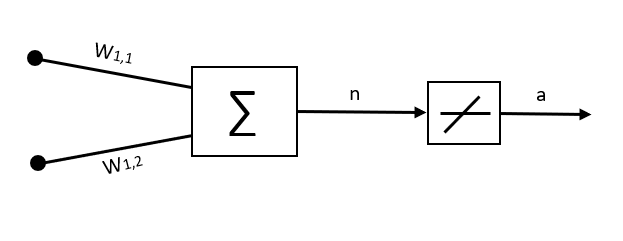
\includegraphics[width=0.5\textwidth]{Problem8_arch.png}
      
    \end{figure}
  \item We need to calculate the various terms of the quadratic function. We know that $F(x) = c - 2x^Th+x^TRx$, where $x = 
    \begin{bmatrix}
      w_{1,1} \\
      w_{1,2} \\
    \end{bmatrix}$. Therefore we need to calculate c, h, and R \\ \\ \\ The expected value of the square of the target is: \\ \\$c = E[t^2] = P(p_1)t_1^2 + P(p_2)t_2^2 + P(p_3)t_3^2 
    = 0.2*26^2 + 0.7*26^2 + 0.1 * (-26)^2 = 26^2 \Rightarrow \bm{c = 676}$ \\ \\ \\The cross-correlation between the input and the target can be calculated: \\ \\
    $h = E[tp] = P(p_1)t_1p_1 + P(p_2)t_2p_2 + P(p_3)t_3p_3 = 0.2*26*
    \begin{bmatrix}
      2 \\
      4 \\
    \end{bmatrix} + 0.7*26*
    \begin{bmatrix}
      4 \\
      2 \\
    \end{bmatrix} + 0.1*(-26)*
    \begin{bmatrix}
      -2 \\
      -2 \\
    \end{bmatrix} = \\
    \begin{bmatrix}
      10.4 \\
      20.8 \\
    \end{bmatrix}+
    \begin{bmatrix}
      72.8 \\
      36.4 \\
    \end{bmatrix}+
    \begin{bmatrix}
      5.2 \\
      5.2 \\
    \end{bmatrix} \Rightarrow \bm{h=}
    \begin{bmatrix}
      \bm{88.4} \\
      \bm{62.4} \\
    \end{bmatrix}$ \\ \\ \\ \\ \\The input correlation matrix R is: \\ \\ $R = E[pp^t] = P(p_1)p_1p_1^T + P(p_2)p_2p_2^T + P(p_3)p_3p_3^T = \\ \\0.2
    \begin{bmatrix}
      2 \\
      4 \\
    \end{bmatrix}\begin{bmatrix}
      2 & 4
    \end{bmatrix} + 0.7
    \begin{bmatrix}
      4 \\
      2 \\
    \end{bmatrix}
    \begin{bmatrix}
      4 & 2
    \end{bmatrix} + 0.1
    \begin{bmatrix}
      -2 \\
      -2 \\
    \end{bmatrix}\begin{bmatrix}
      -2 & -2
    \end{bmatrix} = \\ \\ \\
    \begin{bmatrix}
      0.8 & 1.6 \\
      1.6 & 3.2 \\
    \end{bmatrix} + 
    \begin{bmatrix}
      11.2 & 5.6 \\
      5.6 & 2.8 \\
    \end{bmatrix} + 
    \begin{bmatrix}
      0.4 & 0.4 \\
      0.4 & 0.4 \\
    \end{bmatrix} \Rightarrow \bm{R =}
    \begin{bmatrix}
      \bm{12.4} & \bm{7.6} \\
      \bm{7.6} & \bm{6.4} \\
    \end{bmatrix}$ \\ \\ \\ \\Therefore the mean square error index is: \\ \\$F(x) = 676 - 2
    \begin{bmatrix}
      w_{1,1} & w_{1,2} \\
    \end{bmatrix}
    \begin{bmatrix}
      88.4 \\
      62.4 \\
    \end{bmatrix} + 
    \begin{bmatrix}
      w_{1,1} & w_{1,2} \\
    \end{bmatrix}
    \begin{bmatrix}
      12.4 & 7.6 \\
      7.6 & 6.4 \\
    \end{bmatrix}
    \begin{bmatrix}
      w_{1,1} \\
      w_{1,2} \\
    \end{bmatrix} \\ \\ \\ \Rightarrow \bm{F(x) = 676 - 176.8w_{1,1} - 124.8w_{1,2} + 12.4w_{1,1}^2 + 15.2w_{1,1}w_{1,2} + 6.4w_{1.2}^2}$
    \\ \\ \\ \\In order to find the center of the contours we must find the minimum point, we need to solve: \\ \\
    $x^* = R^{-1}h = 
    \begin{bmatrix}
      12.4 & 7.6 \\
      7.6 & 6.4 \\
    \end{bmatrix}^{-1}
    \begin{bmatrix}
      88.4 \\
      62.4 \\
    \end{bmatrix} = \frac{1}{21.6}
    \begin{bmatrix}
      6.4 & -7.6 \\
      -7.6 & 12.4 \\
    \end{bmatrix}
    \begin{bmatrix}
      88.4 \\
      62.4 \\
    \end{bmatrix} \Rightarrow \bm{x^* \approx} 
    \begin{bmatrix}
      \bm{4.24} \\
      \bm{4.72} \\
    \end{bmatrix}$ \\ \\ \\Thus we have a minimum at $\bm{w_{1,1} \approx 4.24, w_{1,2} \approx 4.72}$ \\ \\ \\ \\
    The resulting contour plot of the MSE is: \\
    \begin{figure}[h]
      \centering
      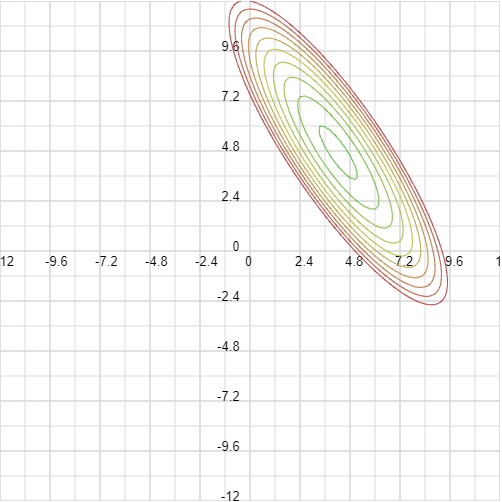
\includegraphics[width=0.5\textwidth]{pr8_b.png}
      
    \end{figure} \\ \\ \\
  \item The decision boundary is defined by the equation:\\ \\ $x^Tp = 0$, where $x = 
    \begin{bmatrix}
      w_{1,1} \\
      w_{1,2} \\
    \end{bmatrix}$ and $p = 
    \begin{bmatrix}
      p_{1,1} \\
      p_{1,2} \\
    \end{bmatrix}$.\\ \\ The optimal decision boundary can be found by using $x^*$ which we already calculated in B. So, by using the weights that minimize the mean square error we get: \\ \\
    $\begin{bmatrix}
      4.24 & 4.72
    \end{bmatrix} 
    \begin{bmatrix}
      p_{1,1} \\
      p_{1,2} \\
    \end{bmatrix} = 0 \Rightarrow 4.24p_{1,1} + 4.72p_{1,2} = 0 \Rightarrow p_{1,2} = -\frac{4.24}{4.72}p_{1,1}$ \\ \\ \\This represents a line in the two-dimensional input space. In order to verify
    that this specific boundary separates the patterns we will calculate $y^{(\bm{p})} = x*^Tp^{(\bm{p})}$, where $\bm{p} = 1,2,3$ \\\\ For $p_1 = 
    \begin{bmatrix}
      2 \\
      4 \\
    \end{bmatrix}$: $y^{(1)} = 4.24*2 + 4.72*4 = 27.36 > 0$ \\ \\ \\For $p_2 = 
    \begin{bmatrix}
      4 \\
      2 \\
    \end{bmatrix}$: $y^{(2)} = 4.24*4 + 4.72*2 = 26.4 > 0$ \\ \\ \\For $p_3 = 
    \begin{bmatrix}
      -2 \\
      -2 \\
    \end{bmatrix}$: $y^{(3)} = 4.24(-2) + 4.72(-2) = -17.88 < 0$ \\ \\ \\ We can see that patterns $p_1$ and $p_2$ have positive outputs indicating that they belong to the category associated with 
    targets $t_1$, $t_2$, whereas pattern $p_3$ has negative output, indicating that it belongs to the category associated with target $t_3$. So, we verified that the patterns are separated in appropriate 
    categories. \\ \\ The optimal decision boundary and the appropriate separation can be seen in the following figure:
    \begin{figure}[h]
      \centering
      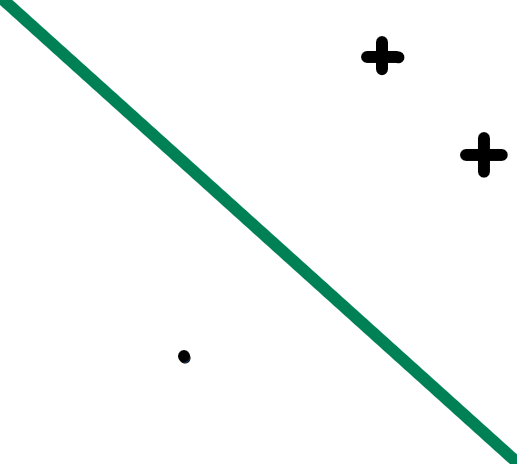
\includegraphics[width=0.2\textwidth]{pr8_c.png}
    \end{figure} 

    
  \item In order for the learning rate of the LMS algorithm to be stable, it must \\be true that: \\ \\${1-2a\lambda_i > -1}$, where ${\lambda_i}$ are the eigenvalues of the R matrix. Knowing that ${\lambda_i > 0}$ the condition on stability is
  ${a < \frac{1}{\lambda_i}}$ or ${0 < a < \frac{1}{\lambda_i}}$. Therefore we get the maximum stable learning rate when ${a = \frac{1}{\lambda_i}}$. 
  \\ \\ $R = \begin{bmatrix}
    12.4 & 7.6 \\
    7.6 & 6.4
  \end{bmatrix} $
  and the eigenvalues of R are ${|R - \lambda*I|}$ \\ \\
  \\$\det \left ( \begin{bmatrix}
    12.4 & 7.6 \\
    7.6 & 6.4
  \end{bmatrix} 
  -\begin{bmatrix}
    \lambda & 0 \\
    0 & \lambda
  \end{bmatrix} \right )  = 
  \det \left (\begin{bmatrix}
    12.4-\lambda & 7.6 \\
    7.6 & 6.4-\lambda
\end{bmatrix} \right ) = (12.4-\lambda)(6.4-\lambda) = \\ \\ \\=\lambda^2 - 18.8\lambda + 21.6$
. So ${\lambda = \frac{47 - \sqrt{1669} }{5}} \approx 1.23$ or ${\lambda = \frac{47 + \sqrt{1669} }{5}} \approx 17.57$. \\ \\ \\In order to get the maximum
learning rate we should choose the minimum lambda. So,
\\ \\ ${a = \frac{1}{\lambda_i} \Rightarrow a= \frac{1}{\frac{47 - \sqrt{1669} }{5}}} \Rightarrow a = \frac{5}{47-\sqrt{1669}} \Rightarrow a \approx 0.814 $\\ \\

If we change the target value from 26 to -26 and from 11 to -11 then the input correlation matrix
$R = E[pp^t] = P(p_1)p_1p_1^T + P(p_2)p_2p_2^T + P(p_3)p_3p_3^T$ will not be affected and so the maximum \\stable learning rate will also remain the same ${a \approx 0.0569}$.

  \item We know that $w(k+1) = w(k) + 2ae(k)p^T(k)$, $w(0) = 
    \begin{bmatrix}
      0 & 0
    \end{bmatrix}$ and $a = 0.05$ \\ \\ Presenting input vector is $p_1$, so one iteration of the Least Mean Square algorithm is: \\ \\
    $a(0) =$ purelin $
    \begin{bmatrix}
      \begin{bmatrix}
        0 & 0
      \end{bmatrix}
      \begin{bmatrix}
        2 \\
        4 \\
      \end{bmatrix}
    \end{bmatrix} = 0$ \\ \\ \\However, $t_1 = 26 \neq 0$, so we need to calculate the error: \\ \\
    $e(0) = t(0) - a(0) = 26 - 0 = 26$ \\ \\ \\ We can now calculate w(1): \\ \\ $w(1) = w(0) +2ae(0)p_1^T = 0 + 2 * 0.05 * 26
    \begin{bmatrix}
      2 & 4
    \end{bmatrix} = 
    \begin{bmatrix}
      5.2 & 10.4
    \end{bmatrix}$
    
  
\end{enumerate}

%Problem 9

\newpage
\noindent \textbf{Problem 9}
\\ \\
Suppose that we have the following two reference patterns and their targets:
\begin{center}
  ${\left \{p1 = \begin{bmatrix} 1 \\ 2\end{bmatrix}, t1 = [-1] \right \} }$, 
  ${\left \{p2 = \begin{bmatrix} -2 \\ 1\end{bmatrix}, t1 = [11] \right \} }$
\end{center}

The vectors are equiprobable. We want to train an ADALINE network without a bias on this data set.
\begin{enumerate} [label=\Alph*]
  \item Sketch the contour plot of the mean square error performance index.
  \item Sketch the optimal decision boundary.
  \item Sketch the trajectory of the LMS algorithm on your contour plot. 
        Assume alearning rate equal to 0.025, and start with initial weights W(0) = [3 1].
\end{enumerate}

\noindent \underline{\textbf{\textit{Solution:}}}

\begin{enumerate} [label=\Alph*]
  \item \leavevmode \begin{center} 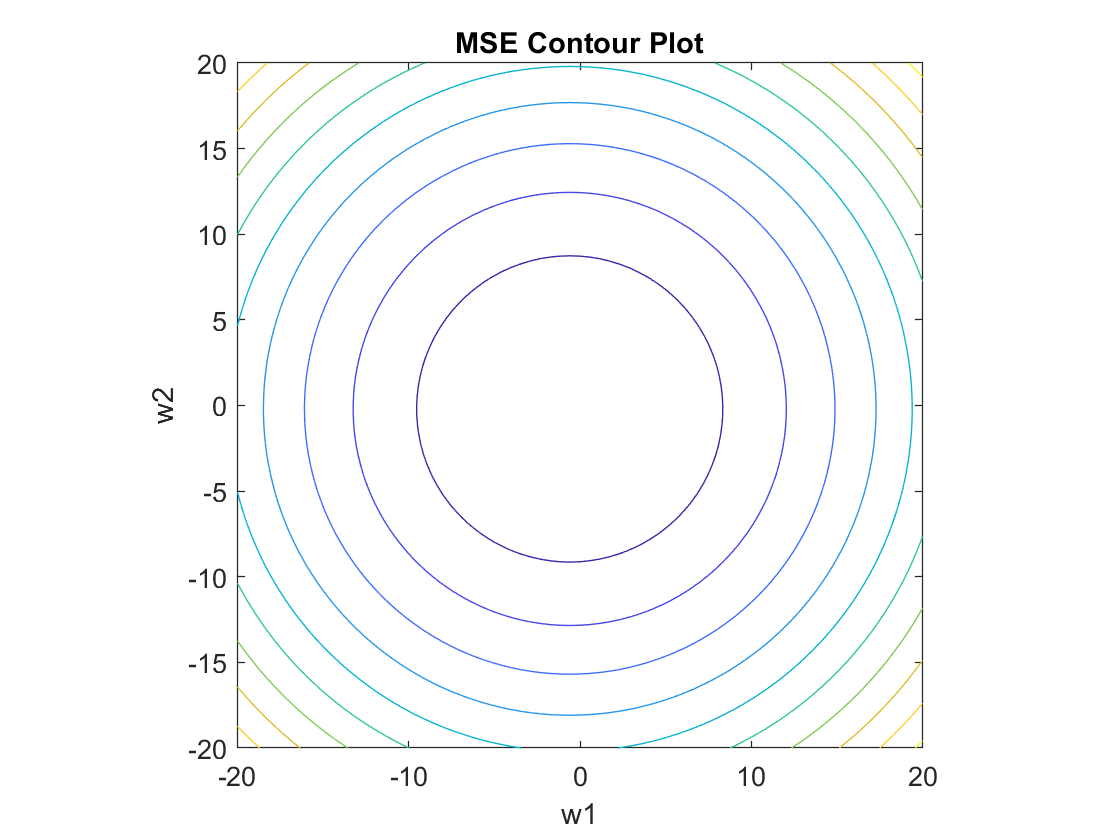
\includegraphics[width=0.8\textwidth]{Problem9_A.png} \end{center}
  \newpage
  \item \leavevmode \begin{center} 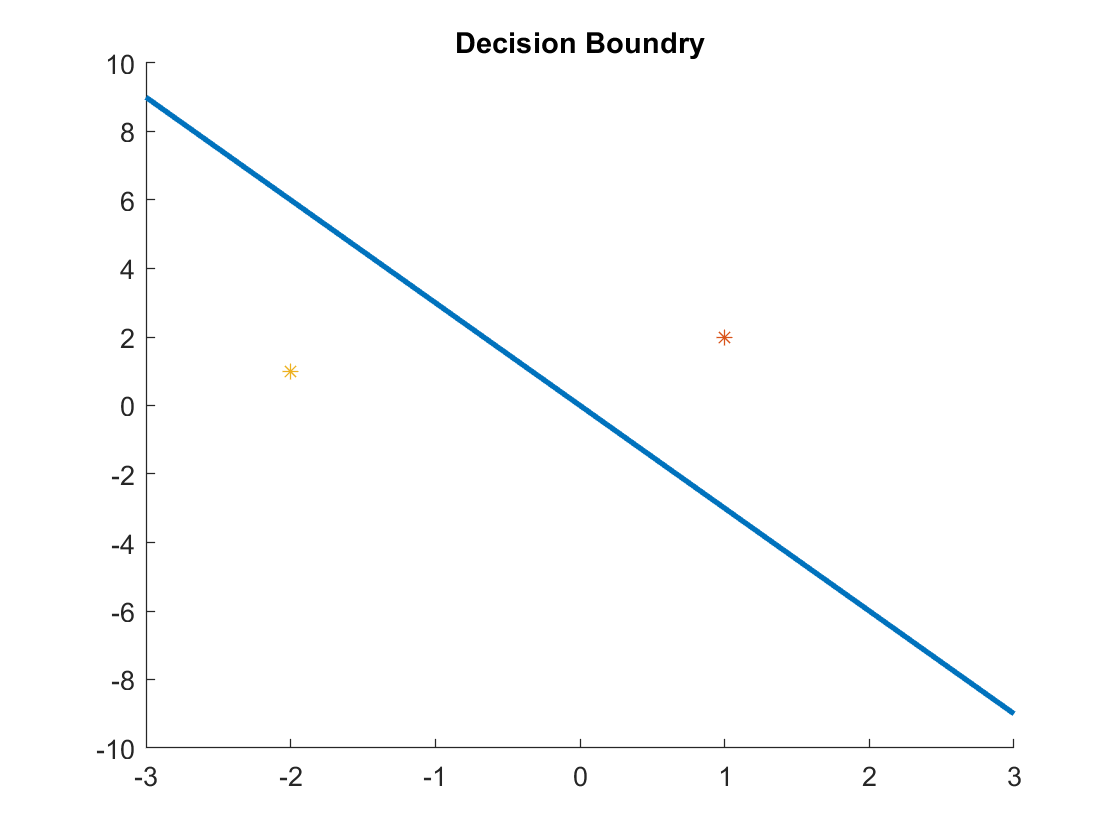
\includegraphics[width=0.7\textwidth]{Problem9_B.png} \end{center} 
  \item \leavevmode \begin{center} 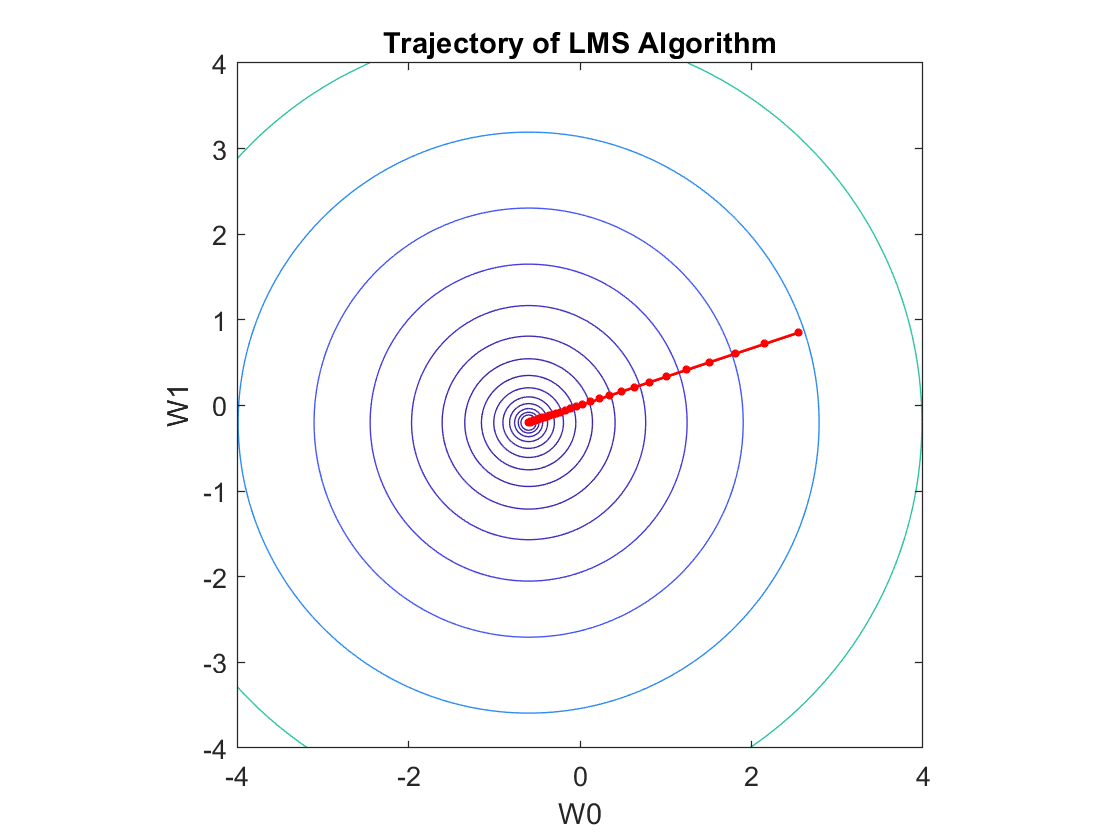
\includegraphics[width=0.9\textwidth]{Problem9_C.png} \end{center} 
\end{enumerate}


%Problem 10
\newpage
\noindent \textbf{Problem 10}

\noindent The patterns (0,0), (0,1), (1,0), (-1,-1) belong to class A and the patterns (2.1,0), (0,-2,5),
(1.6,-1,6) belong to class B. They are equiprobable.
\begin{enumerate} [label=\Alph*]
  \item Draw the patterns in a 2-D diagram. Are the categories linearly separable?
  \item For the aforementioned patterns design the architecture of an ADALINE neural network which will separate the classes.
  \item Starting with initial weights/biases equal to 0.5 calculate the final (after convergence) weights/biases of the ADALINE using the LMS training algorithm
        with learning rate=0.01.\\ \\ \\
\end{enumerate}

\noindent \underline{\textbf{\textit{Solution:}}}
\\ 
\begin{enumerate} [label=\Alph*]
  \item As we can see from the plot the categories are linearly separable. The green line is a hypothetical decision boundary.
  \begin{center} 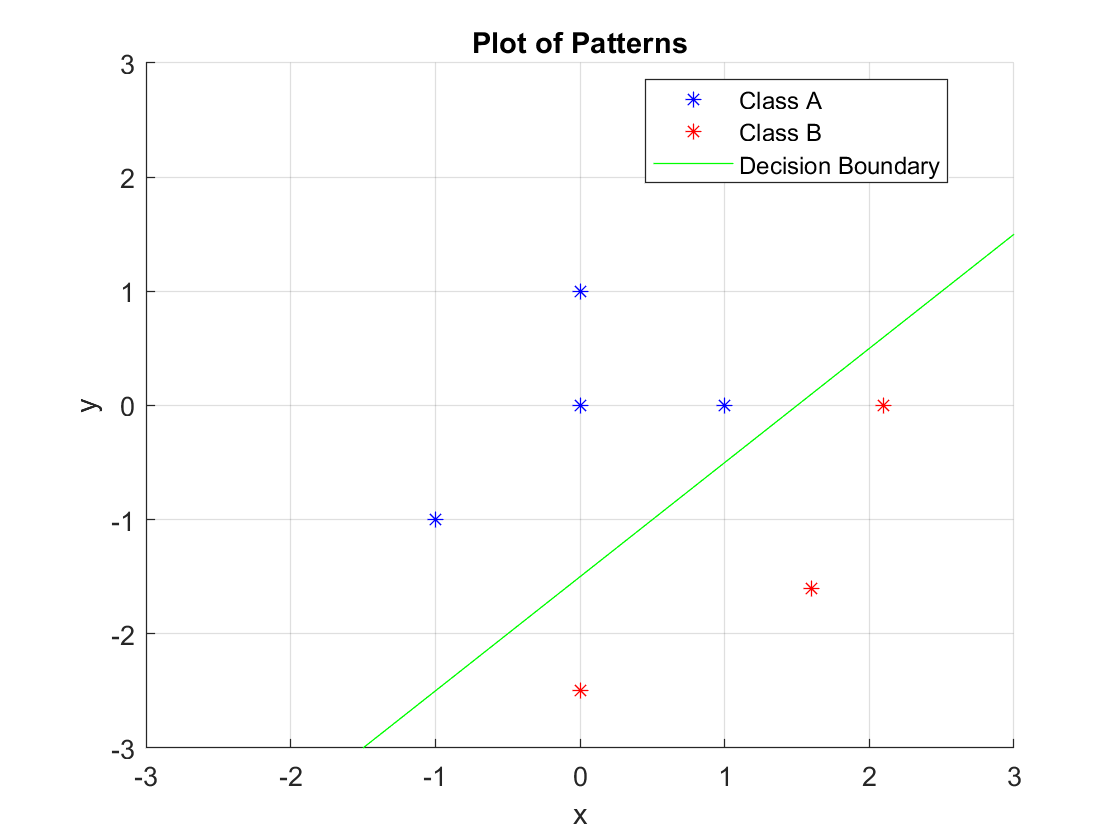
\includegraphics[width=0.9\textwidth]{Problem10_A.png} \end{center}
  \newpage
  \item The architecture of an ADALINE that will separate the classes is: \\
  \begin{figure}[h]
    \centering
    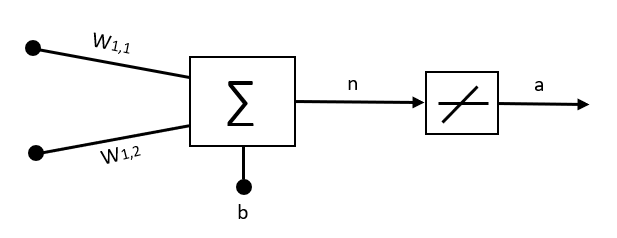
\includegraphics[width=0.6\textwidth]{Problem10.png}
    
  \end{figure}

  \item The final weights are: w1 = -0.655181028588977, w2 = 0.604562000875011 
        and the final bias is b = 0.843268. The decision boundary is shown in the plot:
        \begin{center} 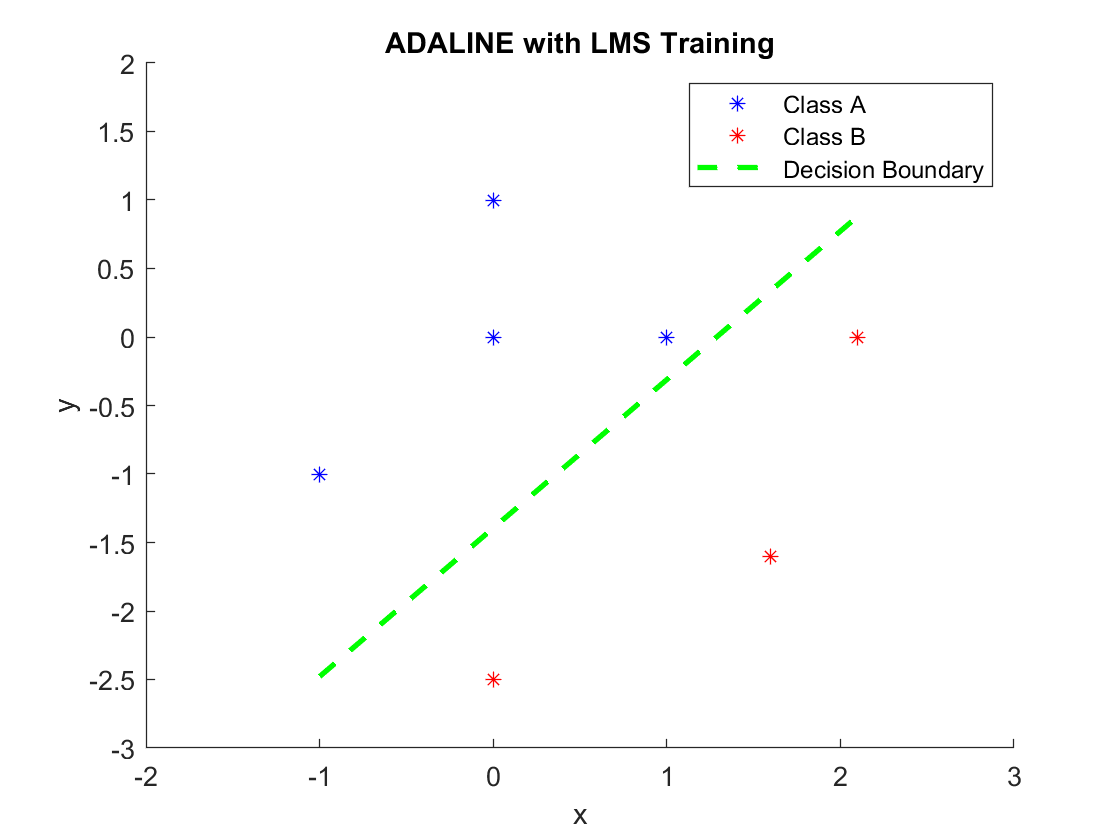
\includegraphics[width=0.9\textwidth]{Problem10_C.png} \end{center}
\end{enumerate}





%Problem 11
\newpage
\noindent \textbf{Problem 11}

\noindent "very" is used as an adjective to reduce vagueness on fuzzy set membership. The interpretation is \\ that if the statement "A is true" has truth value equal to x, then the statement 
"A is very true" has \\ truth value $x^2$, because the "very true" is more demanding. \newline "more or less" is used as an adjective to increase vagueness - the interpretation is that if
"A is true" \\ has truth value x, then "A is more or less true" has truth vlaue $\sqrt{x}$.
\begin{enumerate}
  \item True of false(explain your answer): Let "S" be a fuzzy set. Then "Very S" is a fuzzy subset of "S".
  \item True or false (explain your answer): Let "S" be a fuzzy set. Then "S" is a fuzzy subset of "more or less S".
  \item Using the definitions just given, is it true that "not very S" is a subset of "more or less S", or vice versa, or is it impossible to say?
  \item Is "not more or less S" a subset of "very S", or vice versa, or is it impossible to say? \\ \\
\end{enumerate}


\noindent \underline{\textbf{\textit{Solution:}}}
\\ \\For a set A to be a subset of another set B in X${\rightarrow}$ [0 ... 1], it must be true that  ${I_A(x) \leq I_B(x)}$  for all x in X\\ \\
\begin{enumerate}
  \item True: If "Very S" is ${x^2}$ and "S" is x then ${I_A(x) \leq I_B(x)}$ for every x${\rightarrow}$ [0 ... 1], so "Very S" is a fuzzy subset of "S"
  \\ \begin{center} 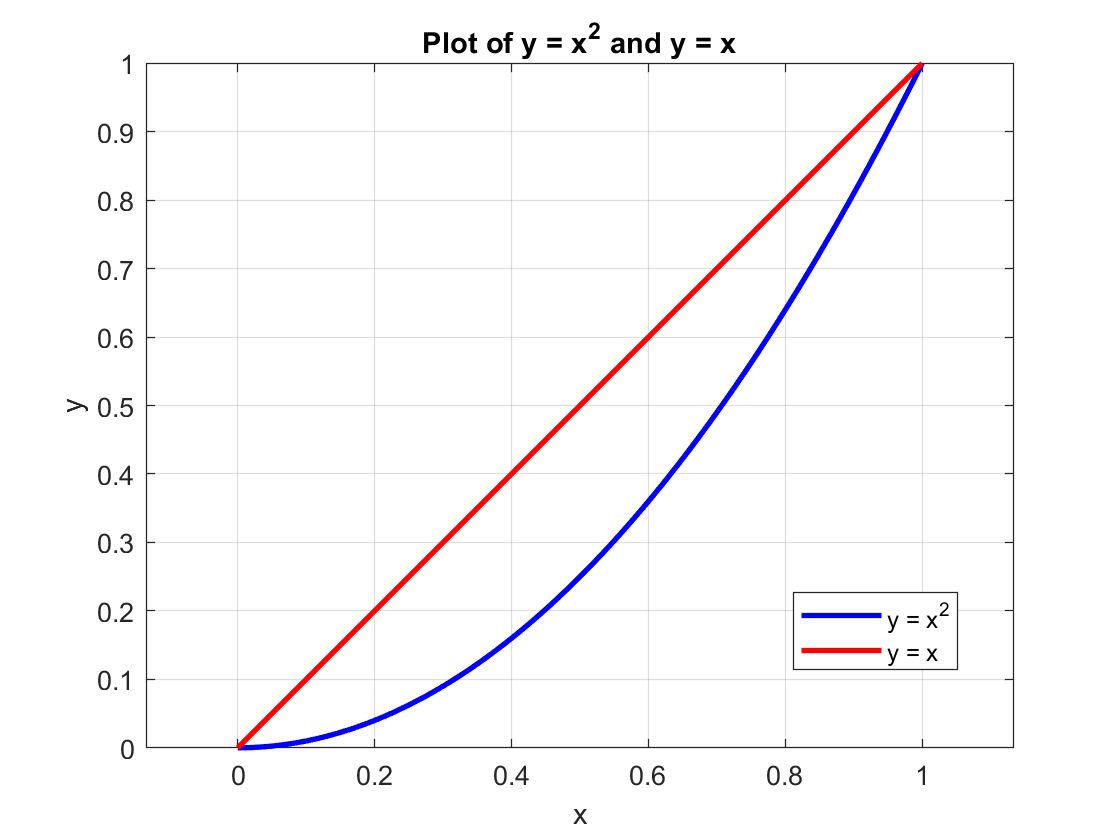
\includegraphics[width=0.45\textwidth]{Problem11_1.png} \end{center}
  \item True: If "S" is x and "more or less S" is ${\sqrt{x}}$ then ${I_A(x) \leq I_B(x)}$ for every x${\rightarrow}$ [0 ... 1], so "S" is a fuzzy subset of "more or less S"
  \\ \begin{center} 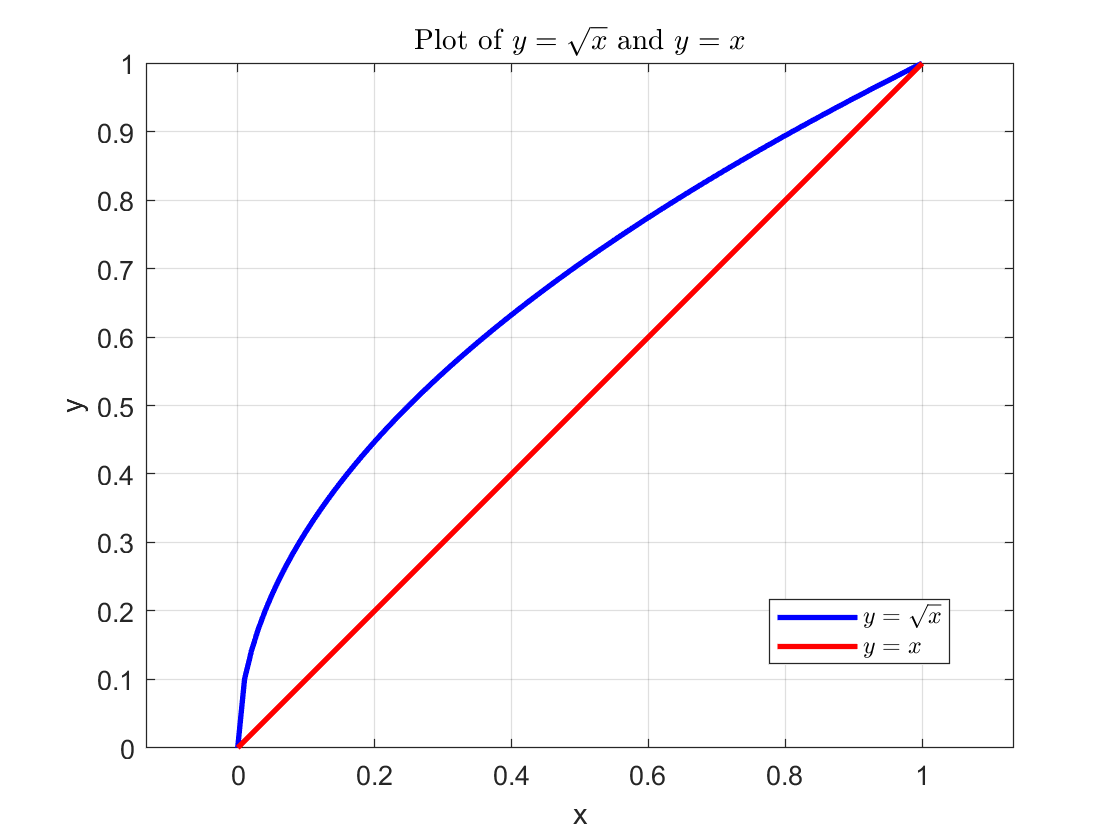
\includegraphics[width=0.45\textwidth]{Problem11_2.png} \end{center}
  \item False: If "Very S" is ${x^2}$ then "not very S" is the complement ${1-x^2}$ and "more or less S" is ${\sqrt{x}}$, so "not very S" is not a subset of "more or less S"
  \\ \begin{center} 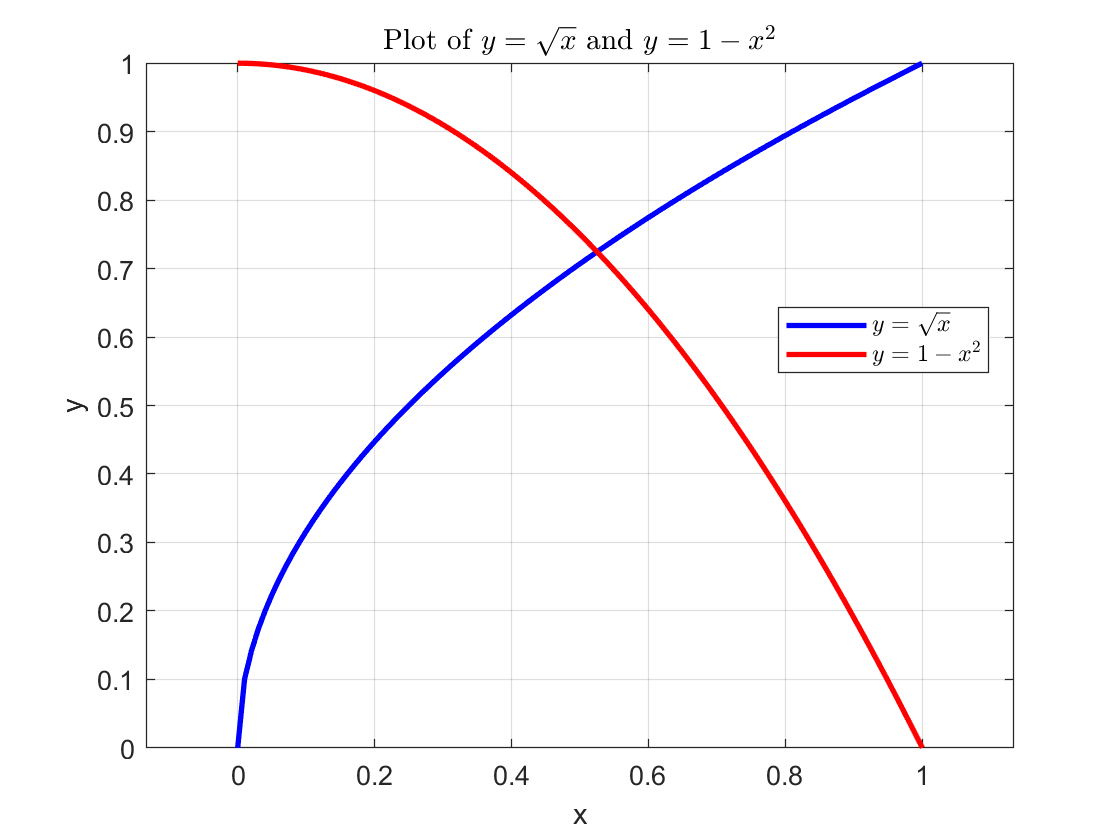
\includegraphics[width=0.45\textwidth]{Problem11_3.png} \end{center} 
  \item False: if "more or less S" is  ${\sqrt{x}}$ then "not more or less S" is the complement ${1-\sqrt{x}}$ and "very S" is ${x^2}$, so "not more or less S" is not a subset of "very S"
  \\ \begin{center} 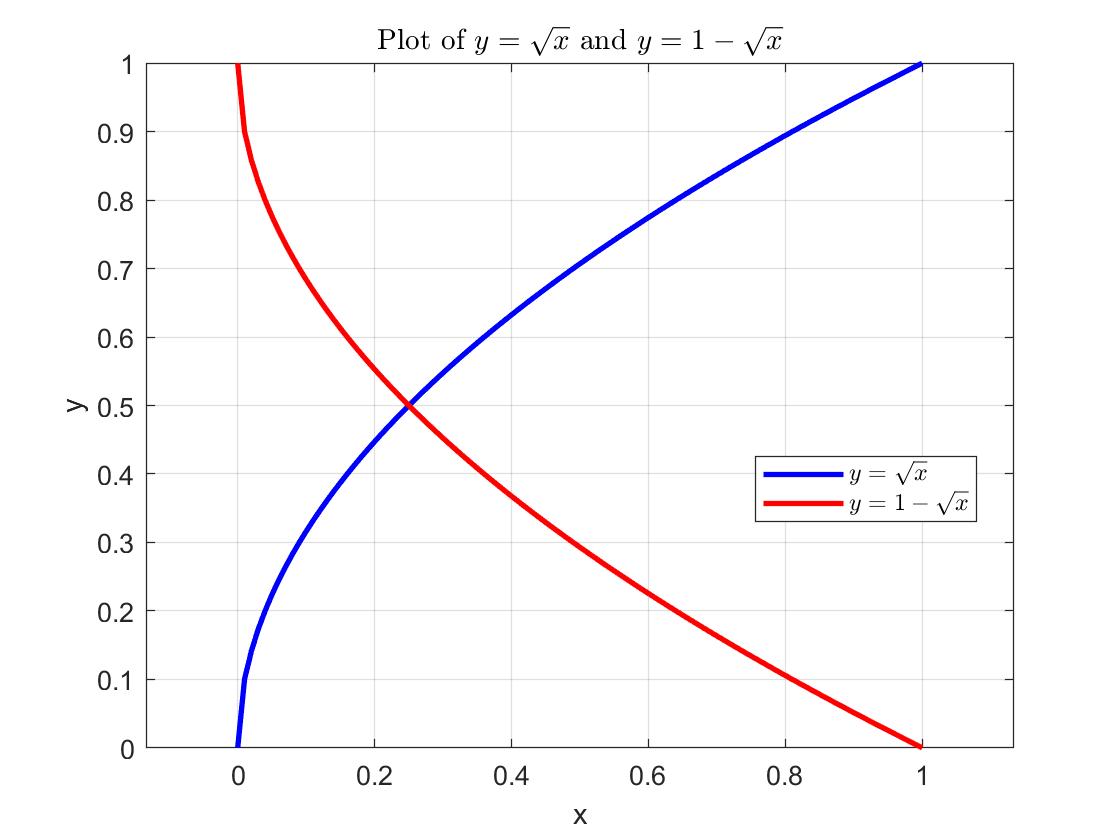
\includegraphics[width=0.45\textwidth]{Problem11_4.png} \end{center}
\end{enumerate}


%Problem 12
\newpage
\noindent \textbf{Problem 12}

\noindent Suppose that A(x) and B(x) have the following truth functions: \\
\noindent \newline
\begin{minipage}{0.45\textwidth}
  \[ A(x) = \begin{cases}
      1 & \text{for } x \leq 2 \\
      1 - \frac{x-2}{3} & \text{for } 2 < x < 5 \\
      0 & \text{for } x \geq 5
  \end{cases} \]
\end{minipage}
\hfill and
\begin{minipage}{0.45\textwidth}
  \[ B(x) = \begin{cases}
      0 & \text{for } x \leq 3 \\
      \frac{x-3}{4} & \text{for } 3 < x < 7 \\
      1 & \text{for } x \geq 7
  \end{cases} \]
\end{minipage}

\noindent \newline \\ \\ Find the values of $x$ for which the proposition not(A(x) OR B(x)) has the maximum possible truth value\\ \\ \\
\underline{\textbf{\textit{Solution:}}}

\begin{figure}[h]
    \centering
    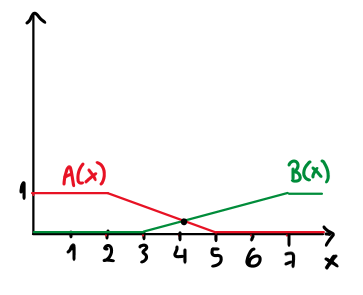
\includegraphics[width=0.4\textwidth]{pr12.png}
    
    
\end{figure}

\noindent \newline We know that the maximum possible truth value is 1 and that not(y) has truth value equal to 1 when y is 0. So in order to 
maximize the truth value of not(A(x) OR B(x)) we should minimize the truth value of A(x) OR B(x). By looking at the graph we can tell that the points that could have the minimum value are the following: \\
\begin{enumerate}
  \item For x = 3, A(3) + B(3) = 0.66 + 0 = 0.66
  \item For x = 5 , A(5) + B(5) = 0 + 0.5 = 0.5
  \item For x = 4.14, A(4.14) + B(4.14) = 0.29 + 0.29 = 0.58
  \item For x = 2, A(2) + B(2) = 1 + 0 = 1
  \item For x = 7, A(7) + B(7) = 0 + 1 = 1
\end{enumerate}
So the maximum truth value for the proposition not(A(x) or B(x)) is for x = 5




\end{document}
